\appendix

\chapter{Supplementary Experimental Figures}
\label{app:supplementary}

This appendix presents the complete figure sets for the paired-granularity analysis (Section~\ref{app:4class}), the layer ablation and complementarity analysis (Section~\ref{app:ablation}), the three-class dynamical characterization (Section~\ref{app:ch6_figs}), and the three-class structure-function coupling analysis (Section~\ref{app:ch7_figs}). These figures support the experimental results reported in Chapters~\ref{chap:arspi_net}--\ref{chap:synthesis}. The reader is referred to the corresponding chapter sections for interpretation and statistical analysis.


%% ═══════════════════════════════════════════════════════════════
%% SECTION A.1: FOUR-CLASS RAW OBSERVATIONS
%% ═══════════════════════════════════════════════════════════════
\section{Four-Class Raw Observations}
\label{app:4class_obs}

The following seven observation sets characterize the SHAPE dataset at four-class resolution (Threat, Mutilation, Cute, Erotic) prior to any classification or clinical analysis. These complement the three-class raw observations presented in Chapter~\ref{chap:arspi_net}, Section~\ref{sec:ch5_raw_obs}, and establish the data landscape for the paired-granularity comparison in Section~\ref{sec:ch5_4class}.

\begin{figure}[H]
    \centering
    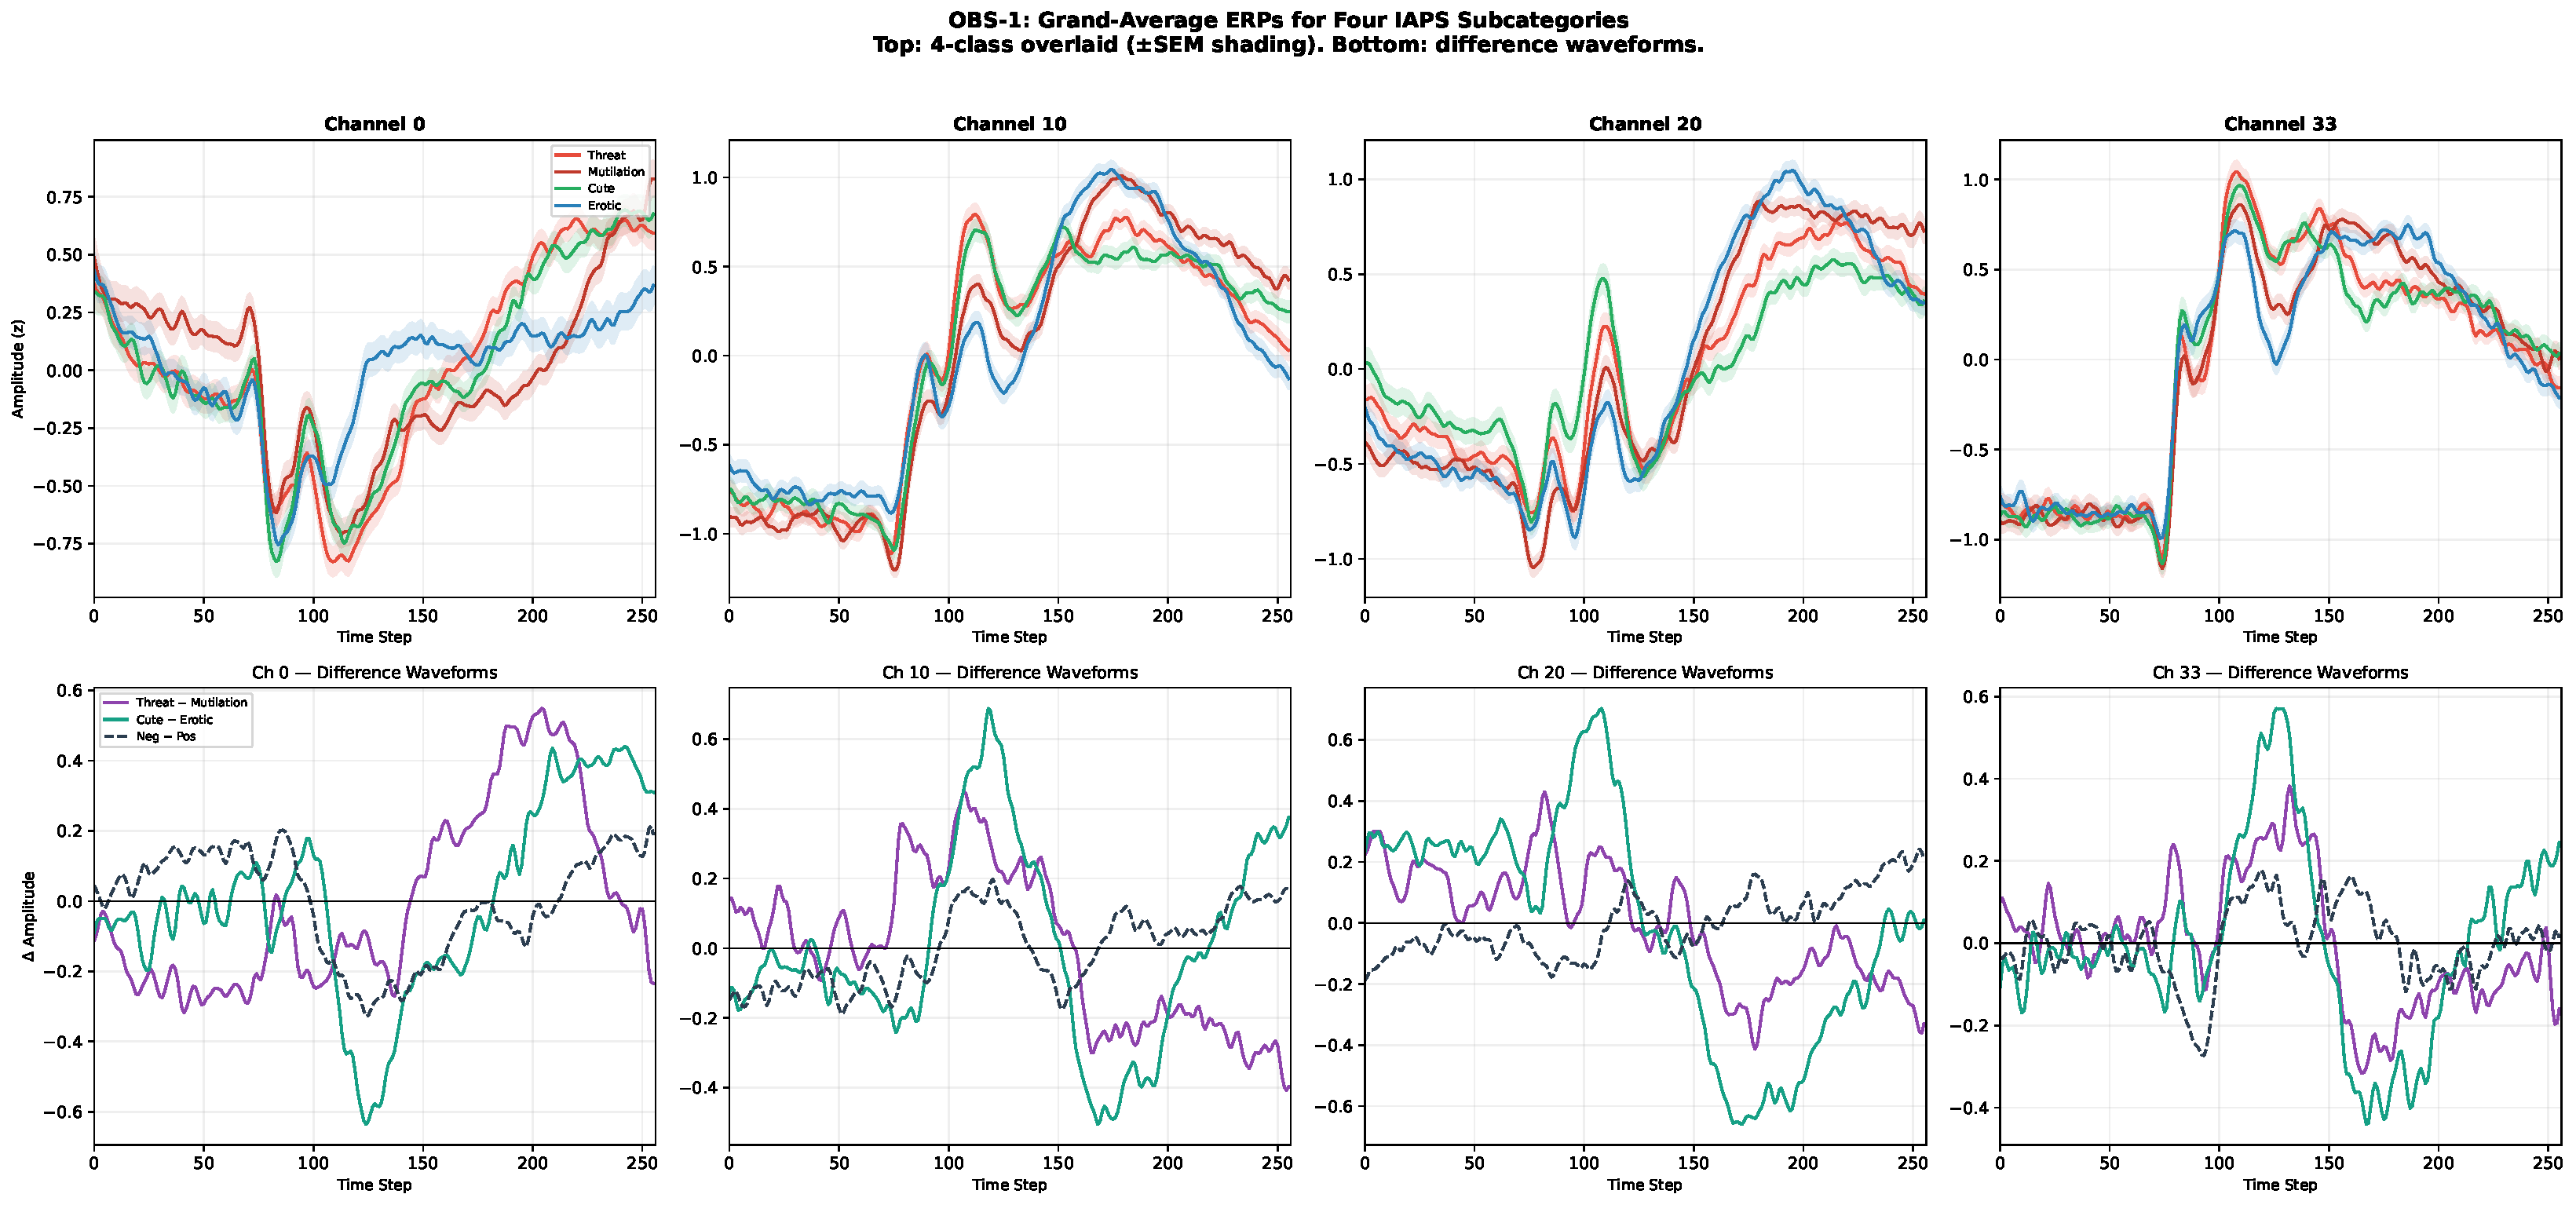
\includegraphics[width=\textwidth]{pictures/appendixA/ch5_4class_obs01_erps.pdf}
    \caption{Grand-average ERPs by category at four-class resolution ($N = 211$). Threat and Mutilation (negative valence) produce larger late positive potentials than Cute and Erotic (positive valence). Within-valence differences are smaller than between-valence differences, consistent with the arousal hierarchy reported in Section~\ref{sec:ch5_4class}.}
    \label{fig:app_4class_obs01}
\end{figure}

\begin{figure}[H]
    \centering
    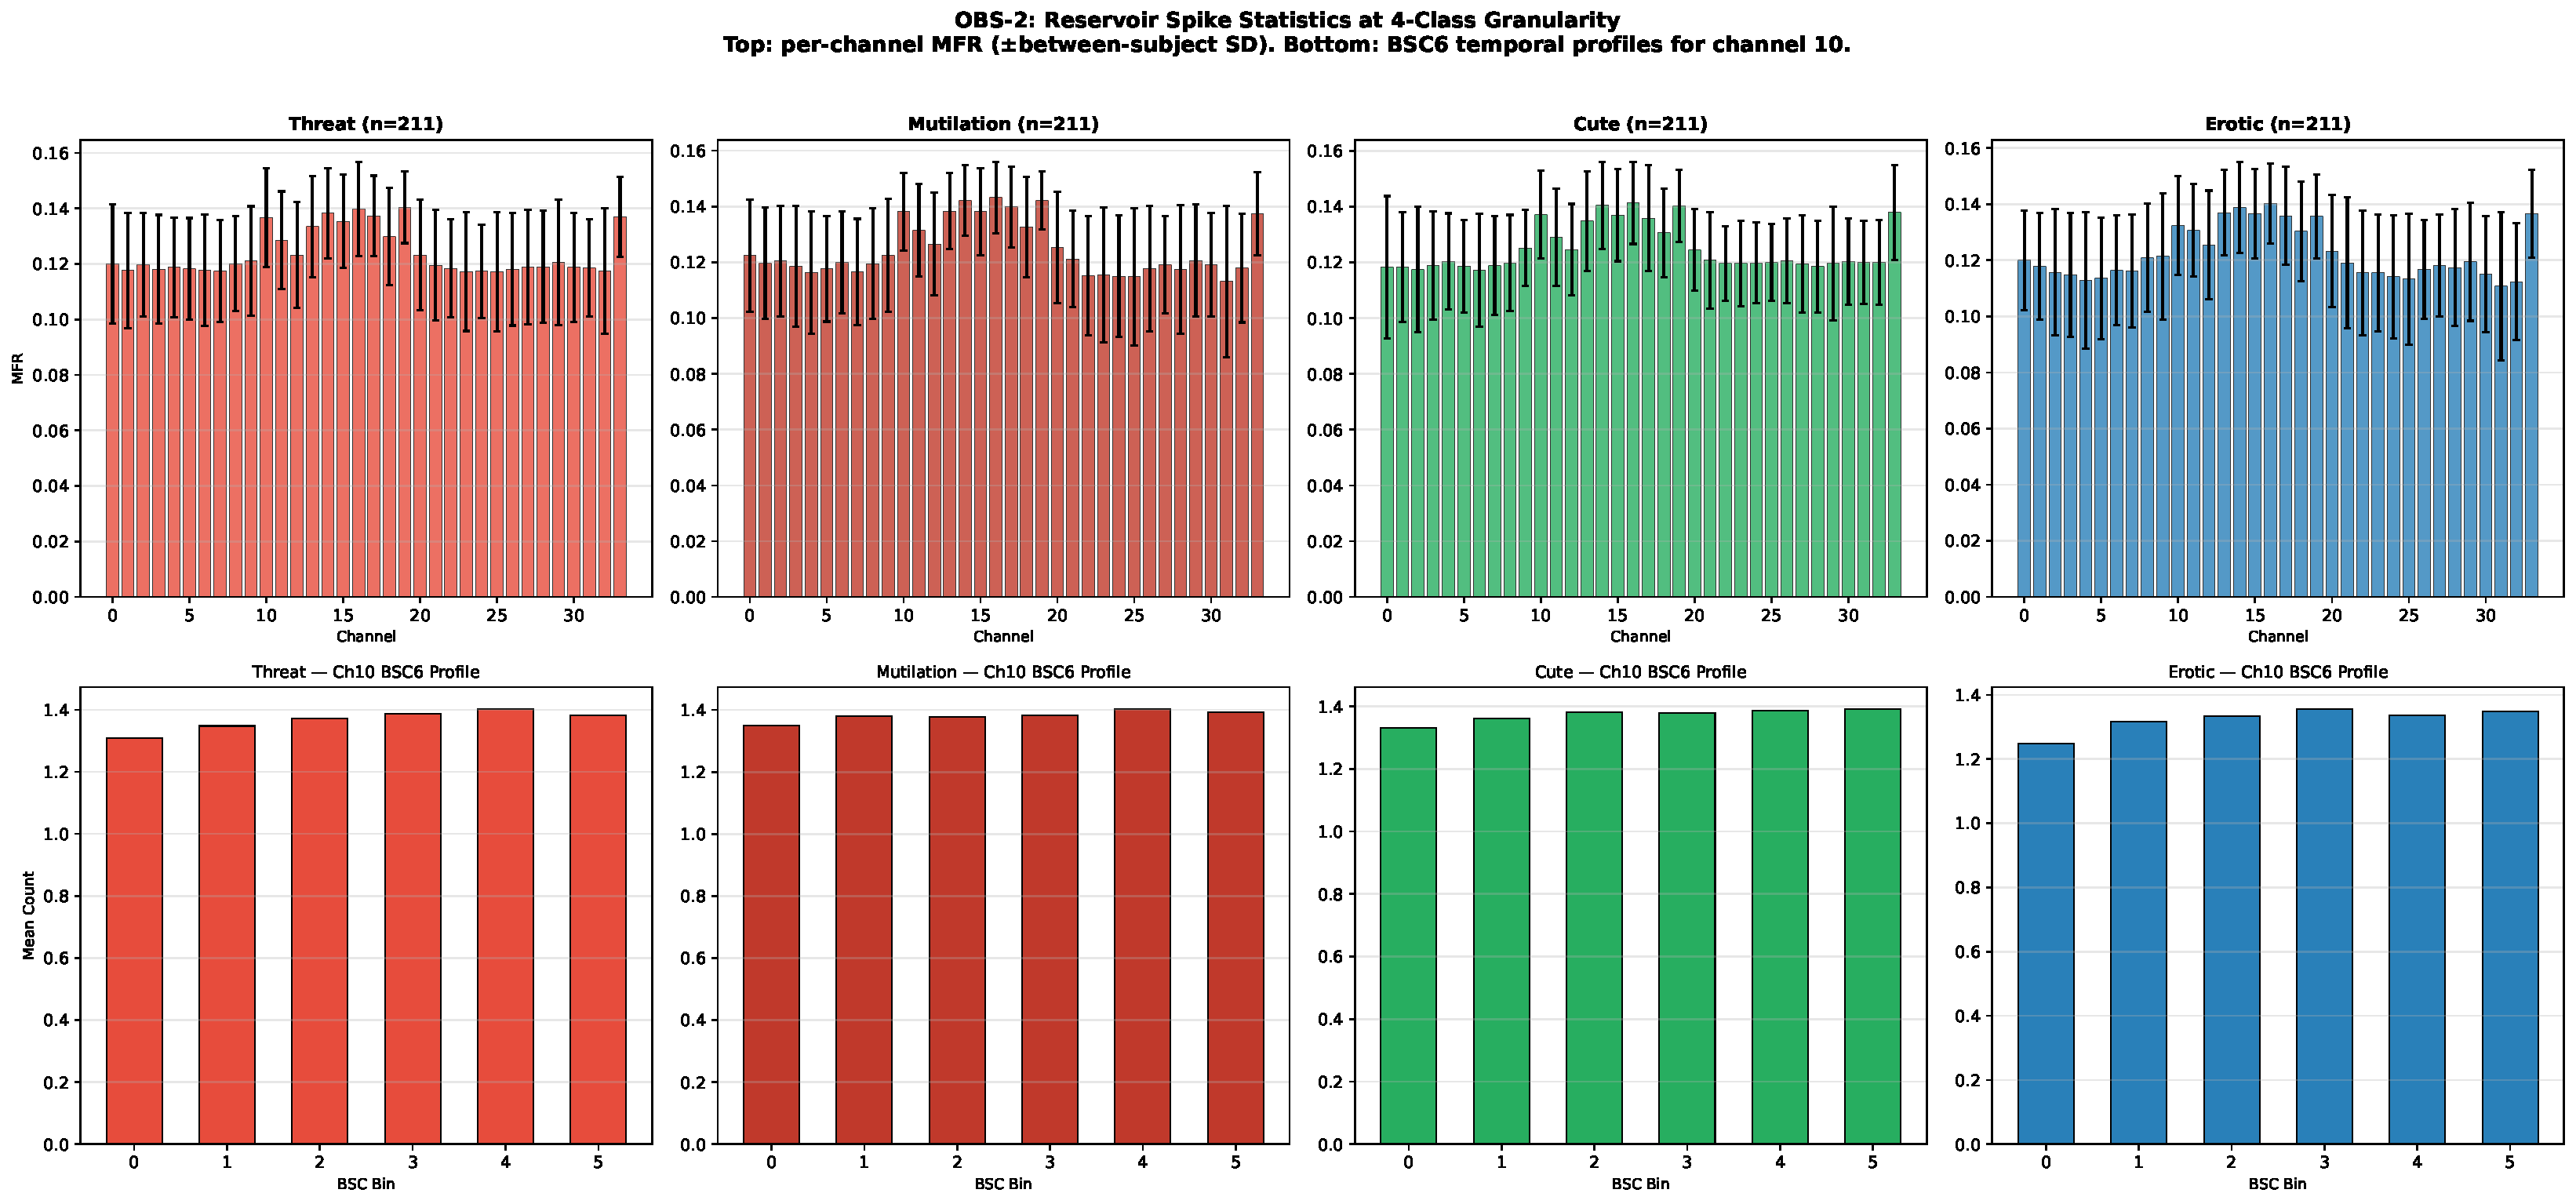
\includegraphics[width=\textwidth]{pictures/appendixA/ch5_4class_obs02_spike_stats.pdf}
    \caption{Reservoir spike statistics at four-class resolution. Per-channel total spike counts and firing rate distributions across the four affective categories. The reservoir produces similar gross activation across categories, with subtle condition-dependent modulations distributed across channels.}
    \label{fig:app_4class_obs02}
\end{figure}

\begin{figure}[H]
    \centering
    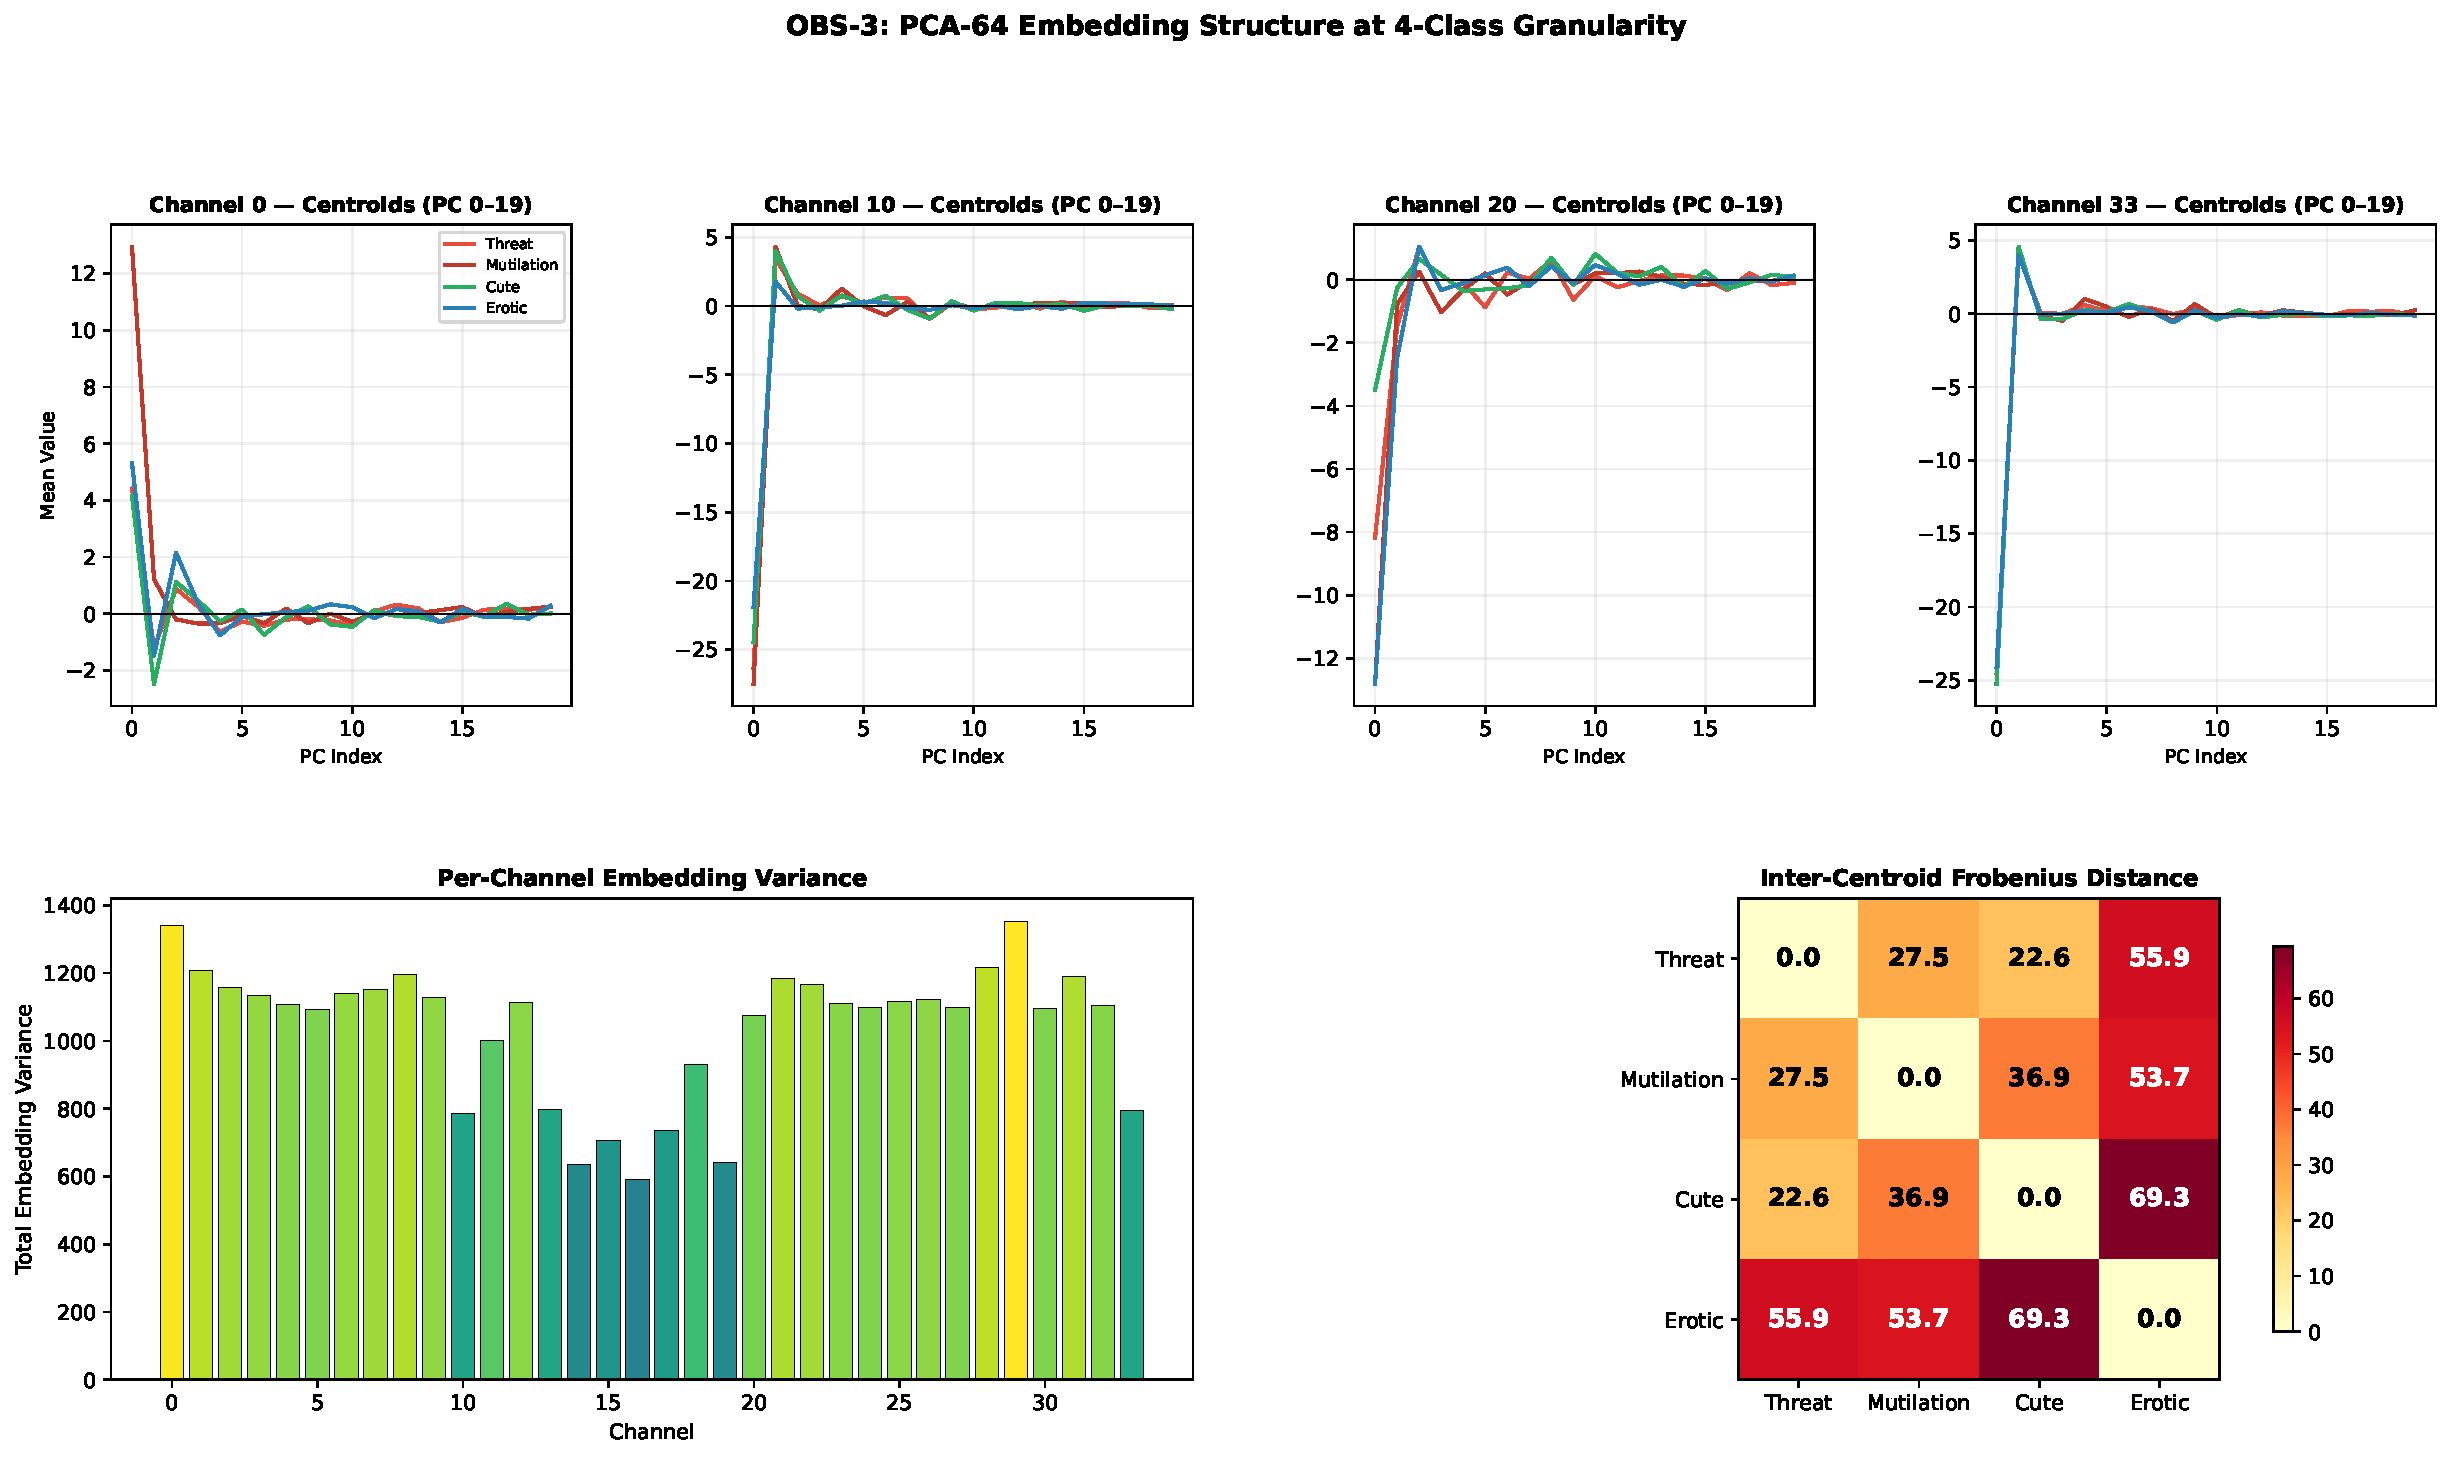
\includegraphics[width=\textwidth]{pictures/appendixA/ch5_4class_obs03_embeddings.pdf}
    \caption{PCA-64 embedding geometry at four-class resolution. Left: PCA-2 projection colored by category shows substantial overlap. Center: projection colored by subject identity shows subject clustering dominates. The four categories are less geometrically separable than the three-class conditions, consistent with the $2.4\%$ condition variance fraction (vs.\ $8.7\%$ at three-class).}
    \label{fig:app_4class_obs03}
\end{figure}

\begin{figure}[H]
    \centering
    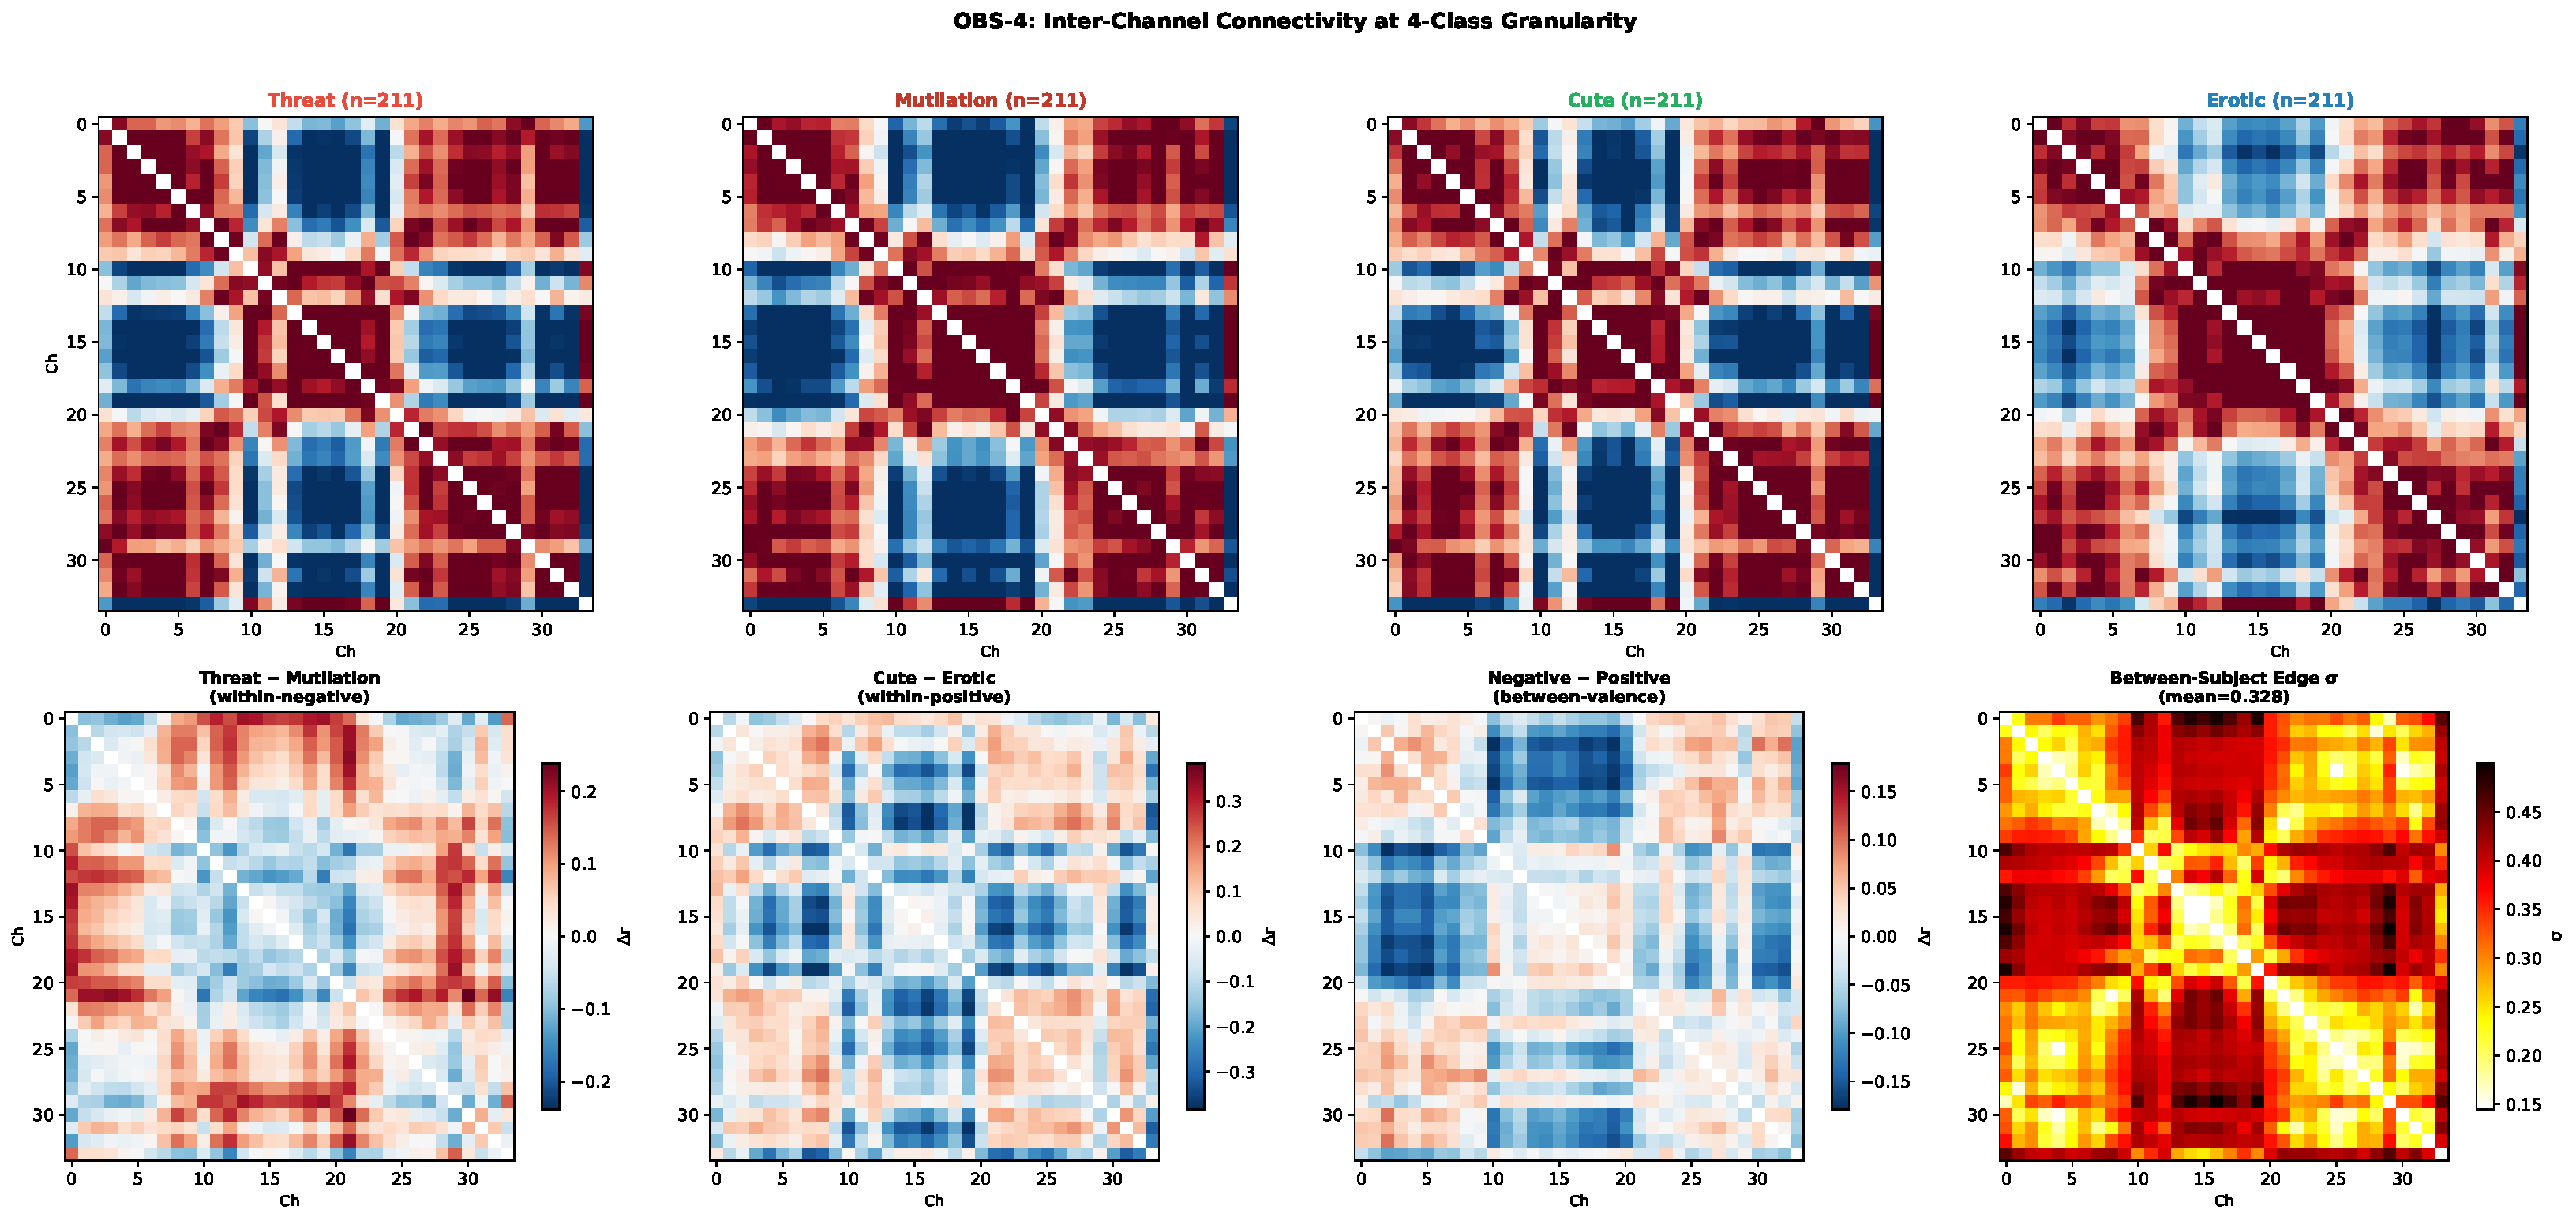
\includegraphics[width=\textwidth]{pictures/appendixA/ch5_4class_obs04_connectivity.pdf}
    \caption{Inter-channel connectivity matrices and graph topology at four-class resolution. The correlation structure is category-dependent but differences are subtle. The $20\%$-density thresholded graphs show similar hub and peripheral structure across all four categories.}
    \label{fig:app_4class_obs04}
\end{figure}

\begin{figure}[H]
    \centering
    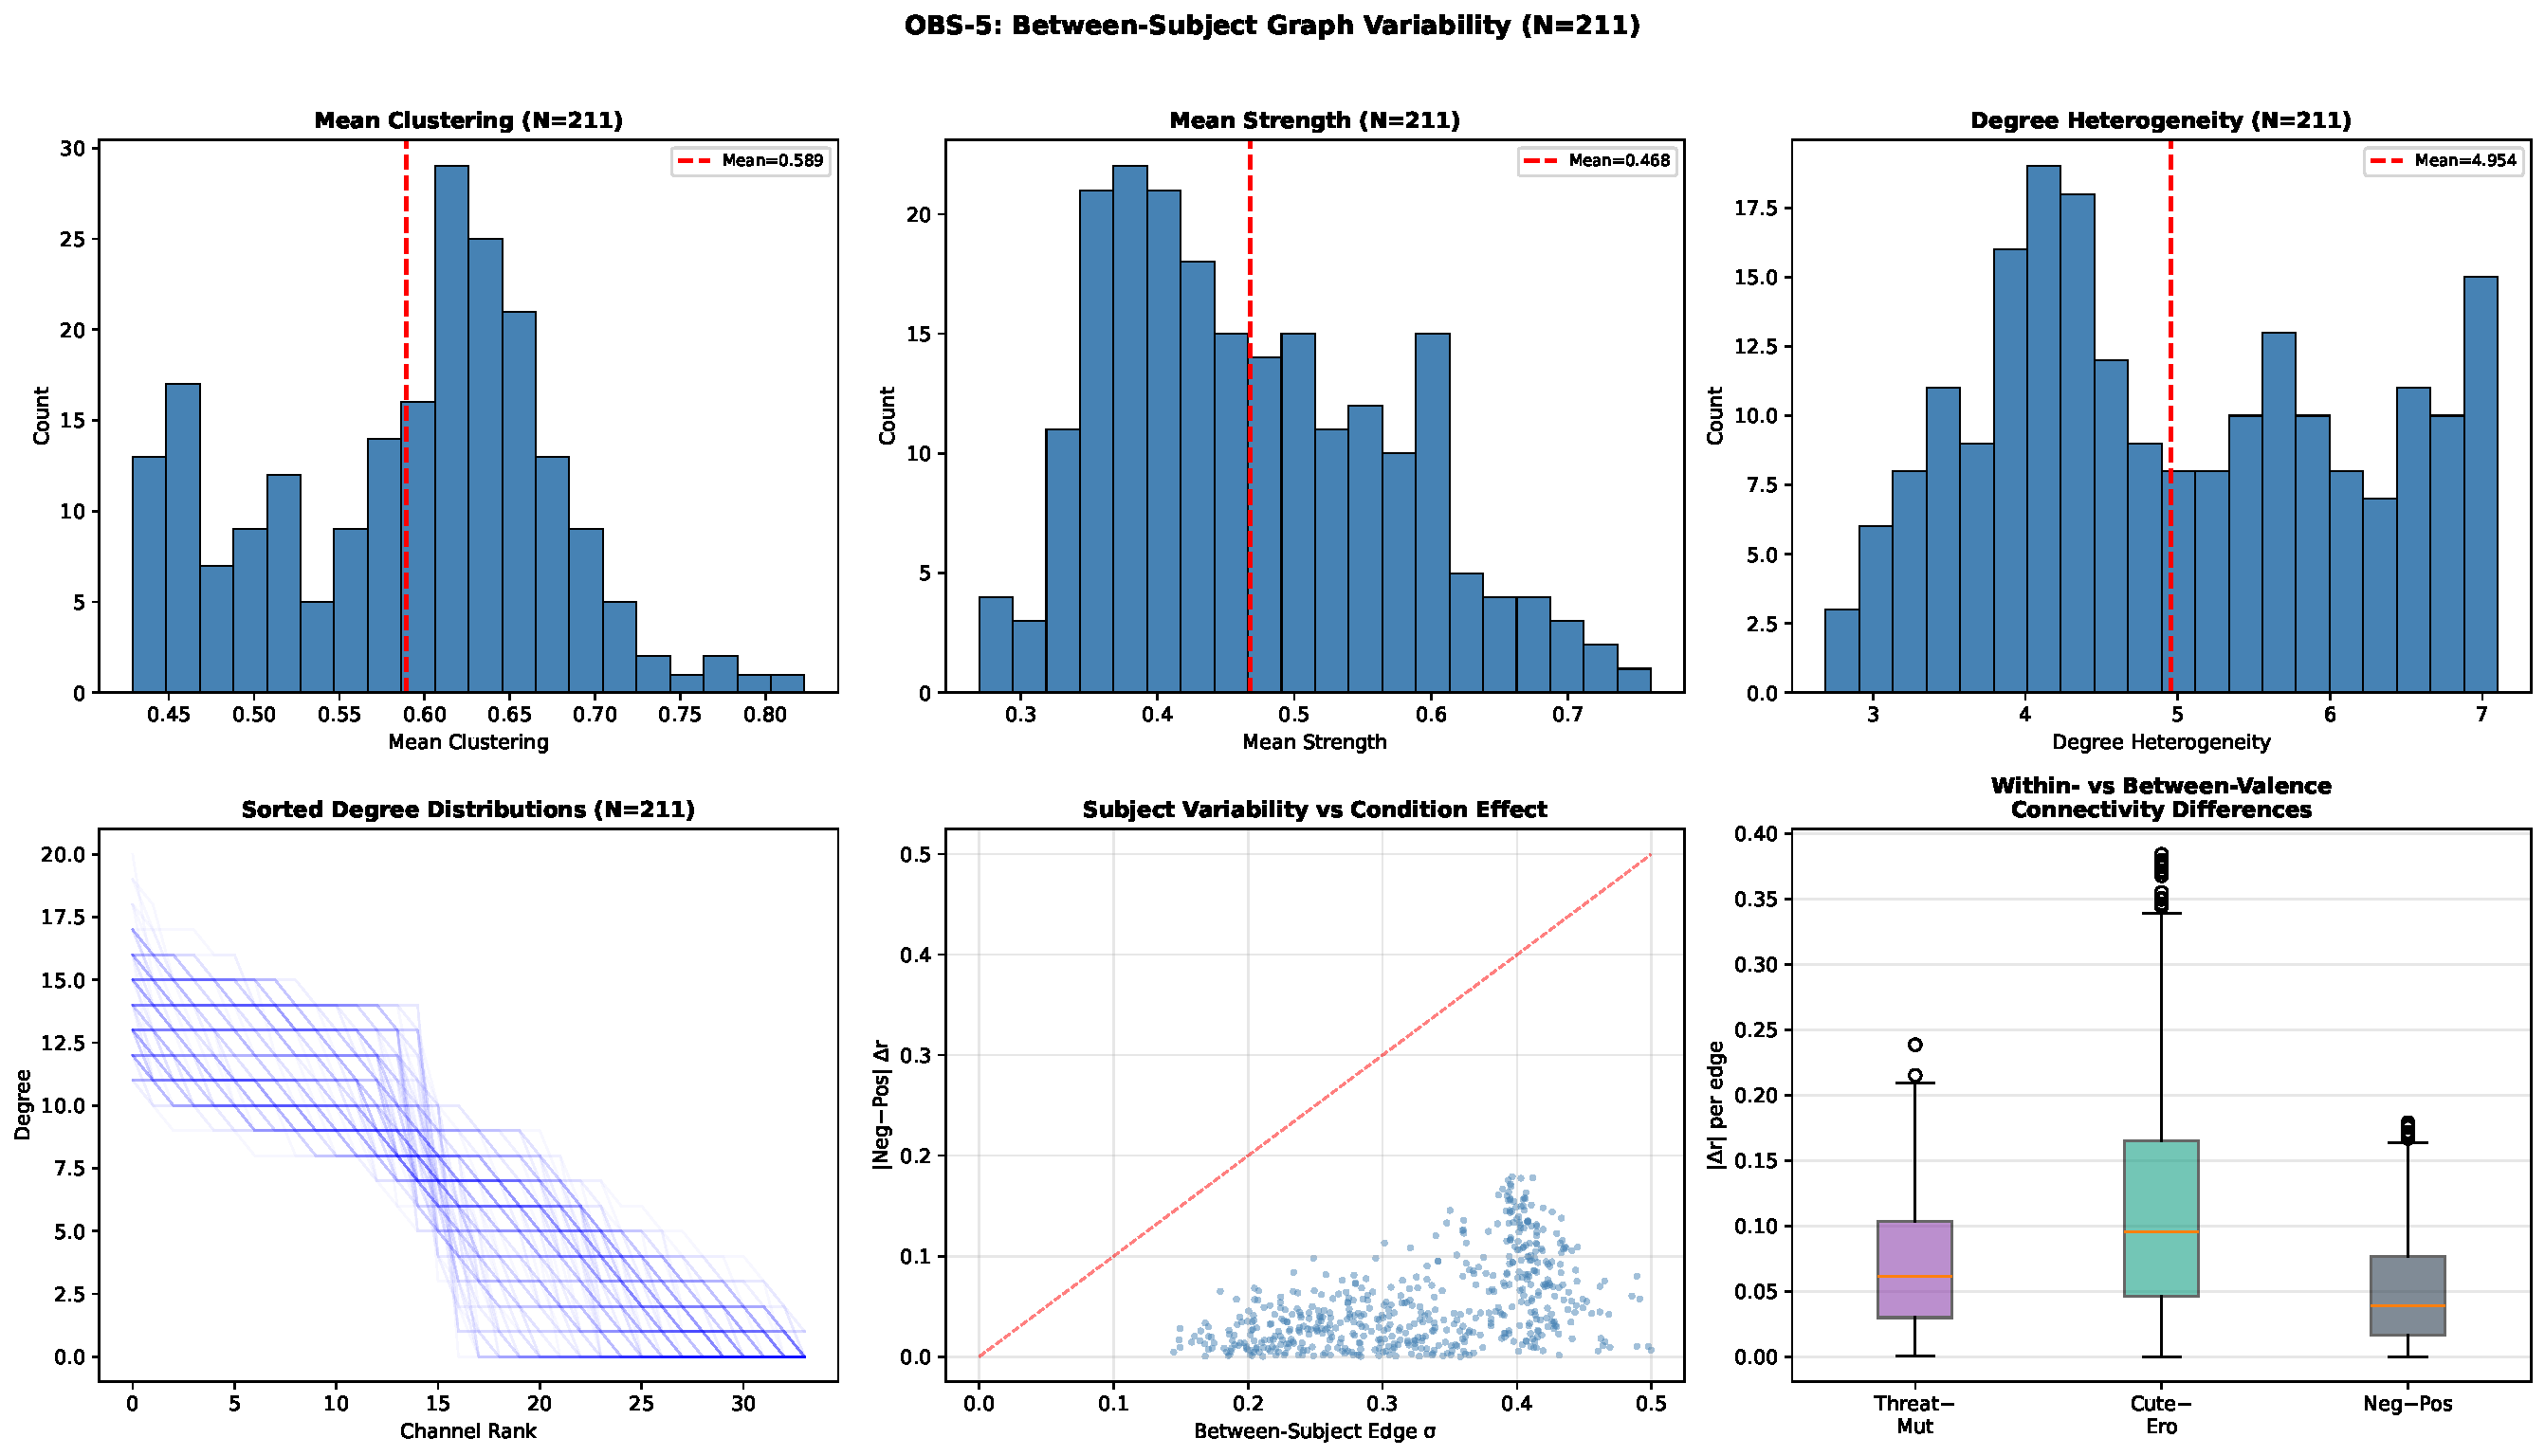
\includegraphics[width=\textwidth]{pictures/appendixA/ch5_4class_obs05_graph_variability.pdf}
    \caption{Between-subject graph variability at four-class resolution. Individual subject graphs show substantial topological diversity. The subject-to-condition signal ratio at four-class ($19.6\times$) is nearly $3\times$ larger than at three-class ($7.2\times$).}
    \label{fig:app_4class_obs05}
\end{figure}

\begin{figure}[H]
    \centering
    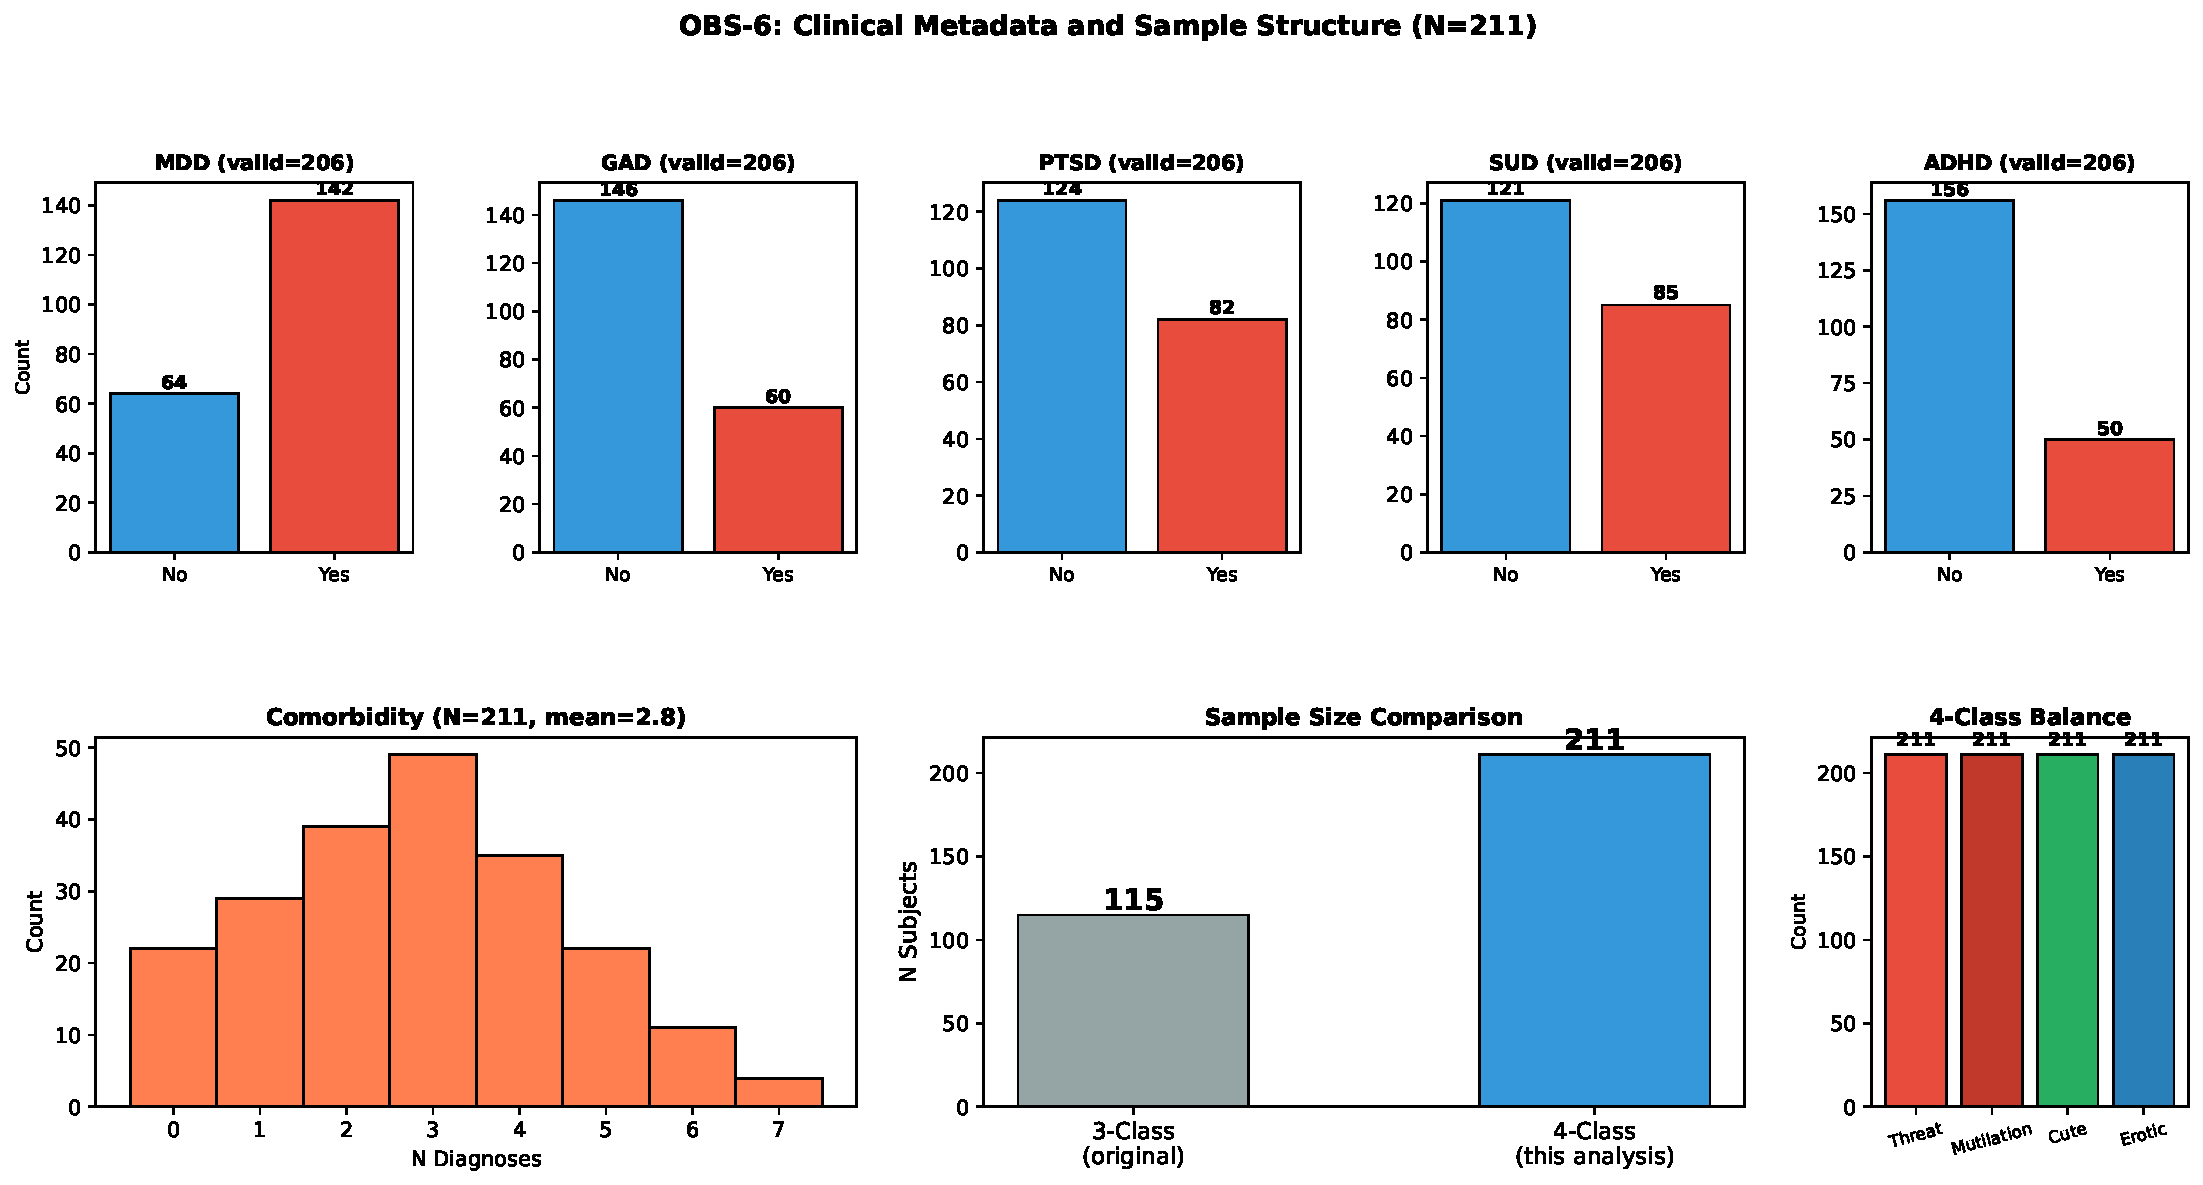
\includegraphics[width=\textwidth]{pictures/appendixA/ch5_4class_obs06_clinical.pdf}
    \caption{Clinical metadata coverage for the four-class analysis ($N = 211$ subjects, $844$ observations). Group sizes and diagnostic distributions are identical to the three-class analysis because the same subjects contribute to both granularities.}
    \label{fig:app_4class_obs06}
\end{figure}

\begin{figure}[H]
    \centering
    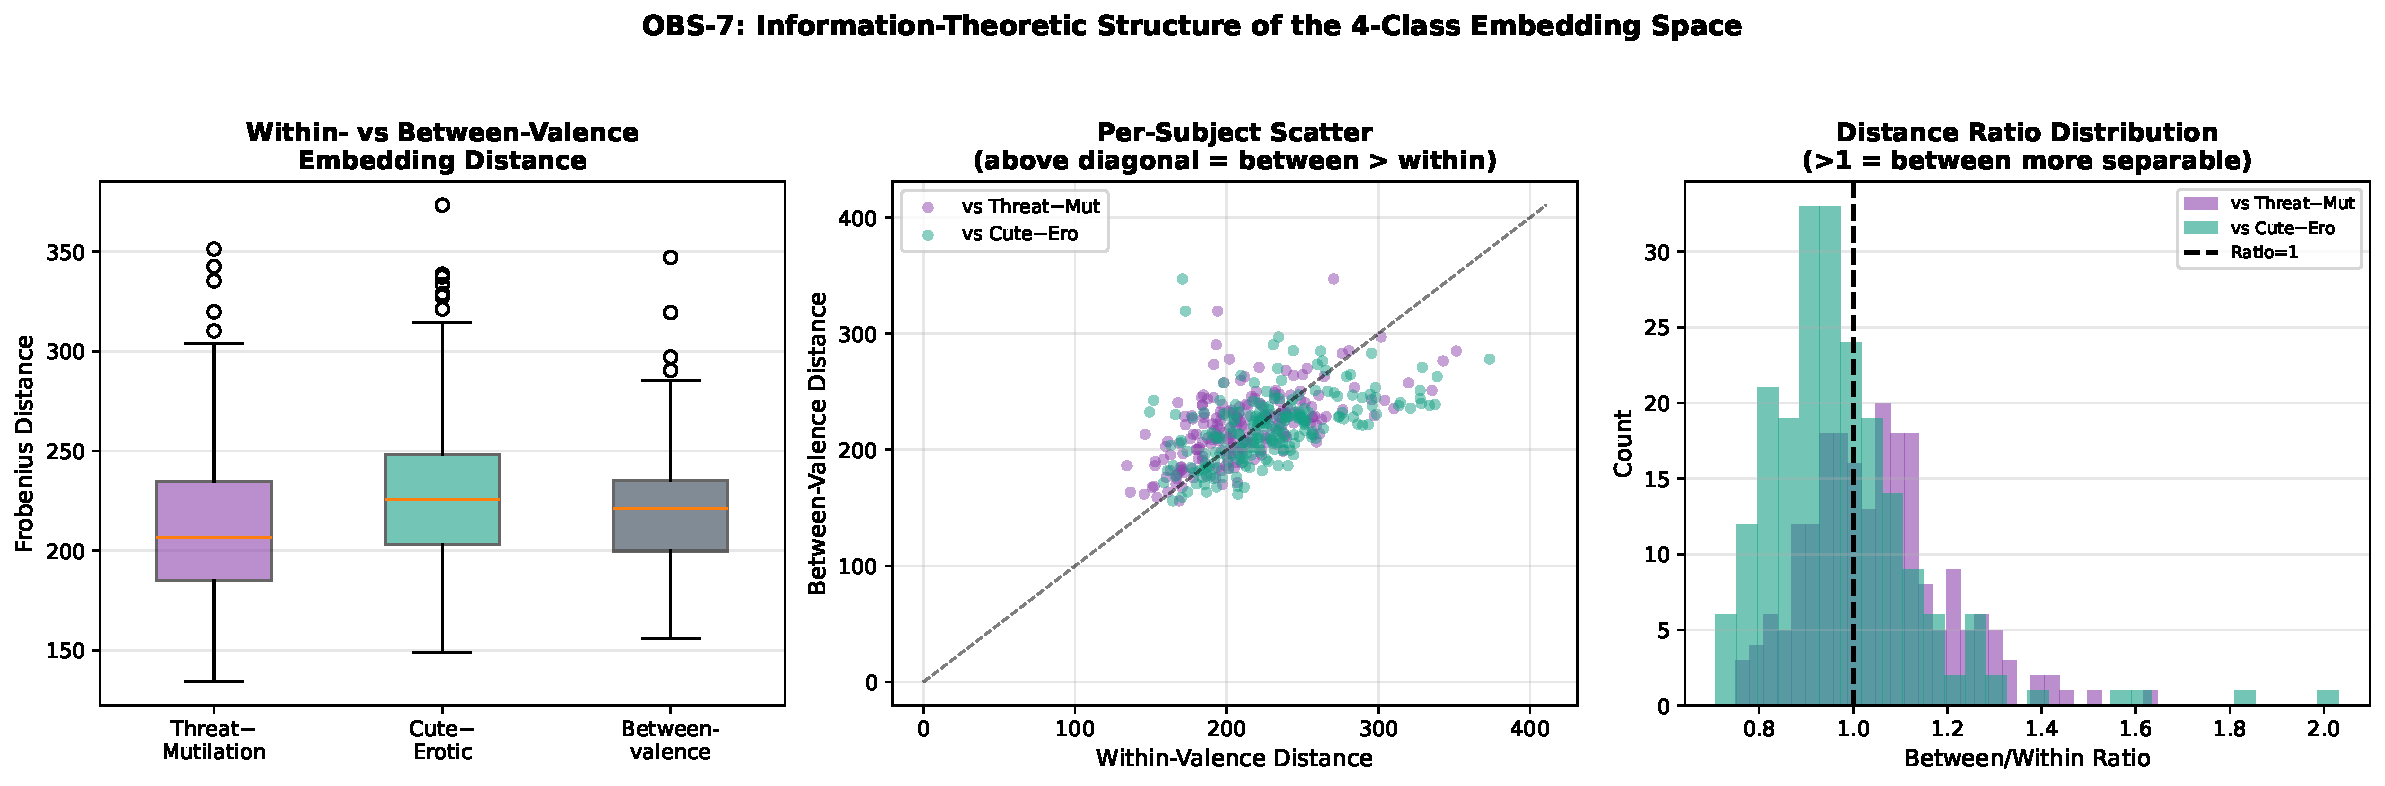
\includegraphics[width=\textwidth]{pictures/appendixA/ch5_4class_obs07_distance_structure.pdf}
    \caption{Within-valence versus between-valence distance structure at four-class resolution. The pairwise embedding distances reveal that within-valence category pairs (Threat--Mutilation, Cute--Erotic) are closer in embedding space than between-valence pairs, consistent with the classification finding that within-valence discriminations are harder than between-valence discriminations for the reservoir representation.}
    \label{fig:app_4class_obs07}
\end{figure}


%% ═══════════════════════════════════════════════════════════════
%% SECTION A.2: FOUR-CLASS EXPERIMENTAL RESULTS
%% ═══════════════════════════════════════════════════════════════
\section{Four-Class Classification and Clinical Results}
\label{app:4class}

The following nine figures present the complete four-class experimental results supporting the paired-granularity analysis in Chapter~\ref{chap:arspi_net}, Section~\ref{sec:ch5_4class}.

\begin{figure}[H]
    \centering
    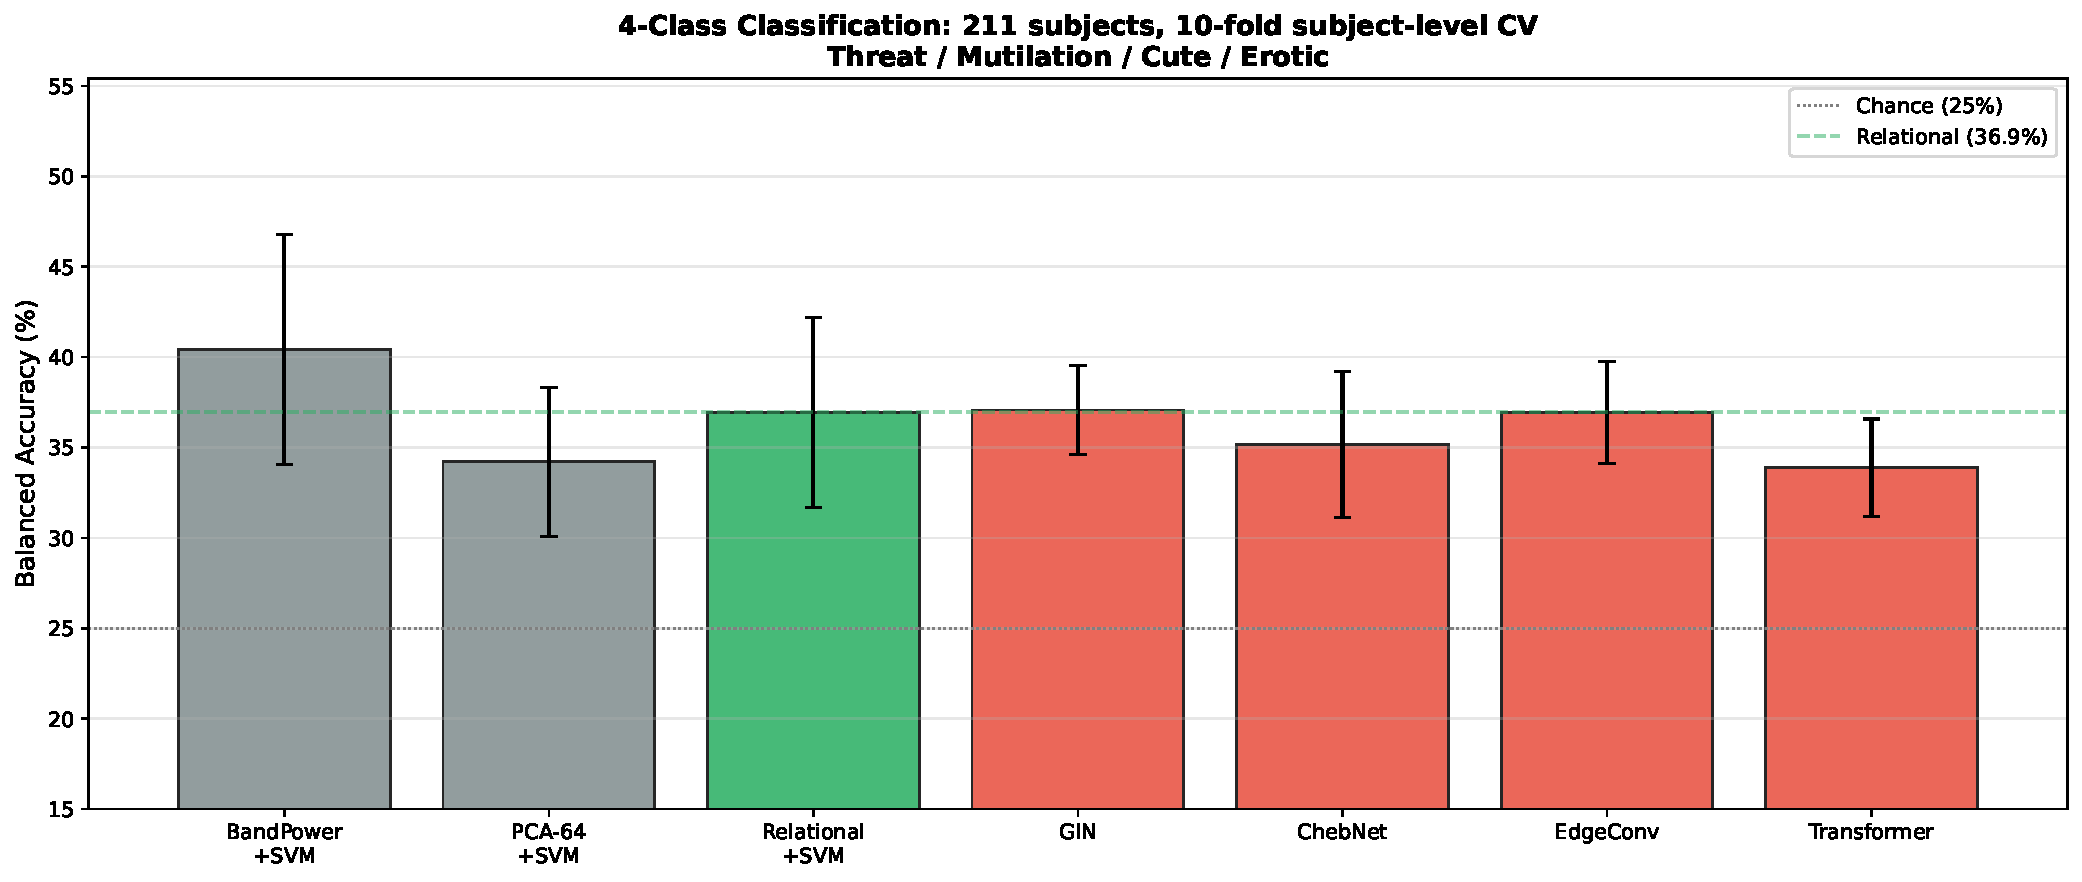
\includegraphics[width=\textwidth]{pictures/appendixA/ch5_4class_fig01_gnn_comparison.pdf}
    \caption{Classification comparison at four-class resolution ($N = 211$, $844$ observations). Band-power features ($40.4\%$) outperform the reservoir embedding ($34.2\%$), reversing the three-class hierarchy where the reservoir leads by $+12.5$~pp. No GNN architecture exceeds the non-propagated baseline, replicating the regime boundary from three-class.}
    \label{fig:app_4class_fig01}
\end{figure}

\begin{figure}[H]
    \centering
    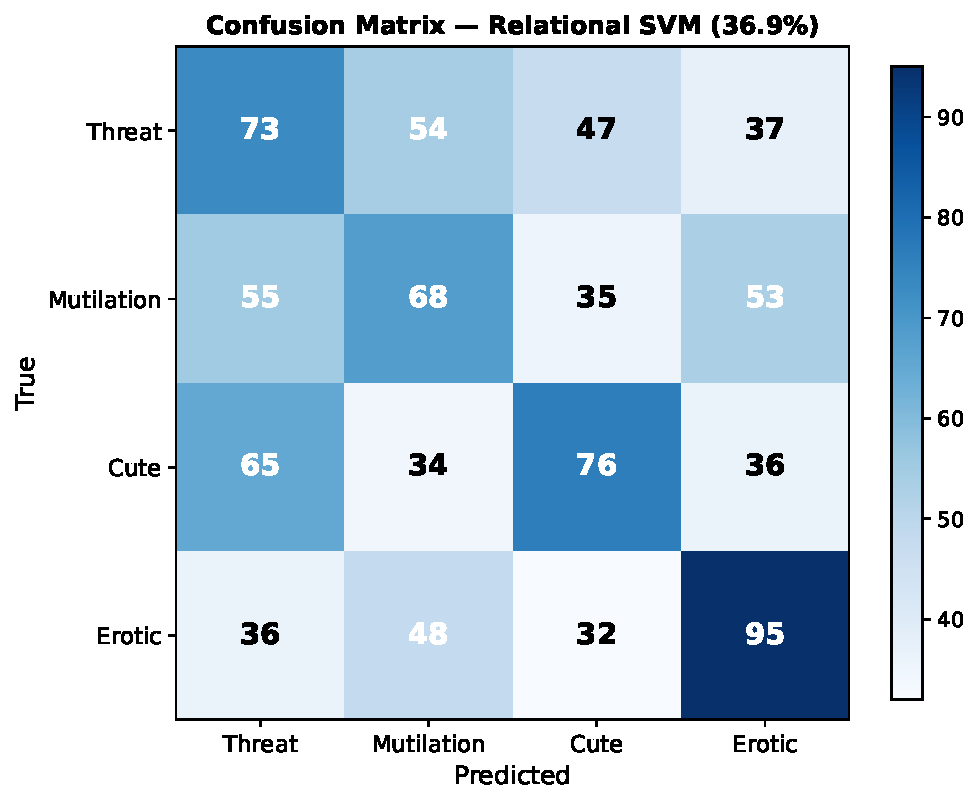
\includegraphics[width=\textwidth]{pictures/appendixA/ch5_4class_fig02_confusion_matrix.pdf}
    \caption{Confusion matrix at four-class resolution. Within-valence errors (Threat$\leftrightarrow$Mutilation, Cute$\leftrightarrow$Erotic) account for $33\%$ of all misclassifications, consistent with the valence-organized embedding geometry.}
    \label{fig:app_4class_fig02}
\end{figure}

\begin{figure}[H]
    \centering
    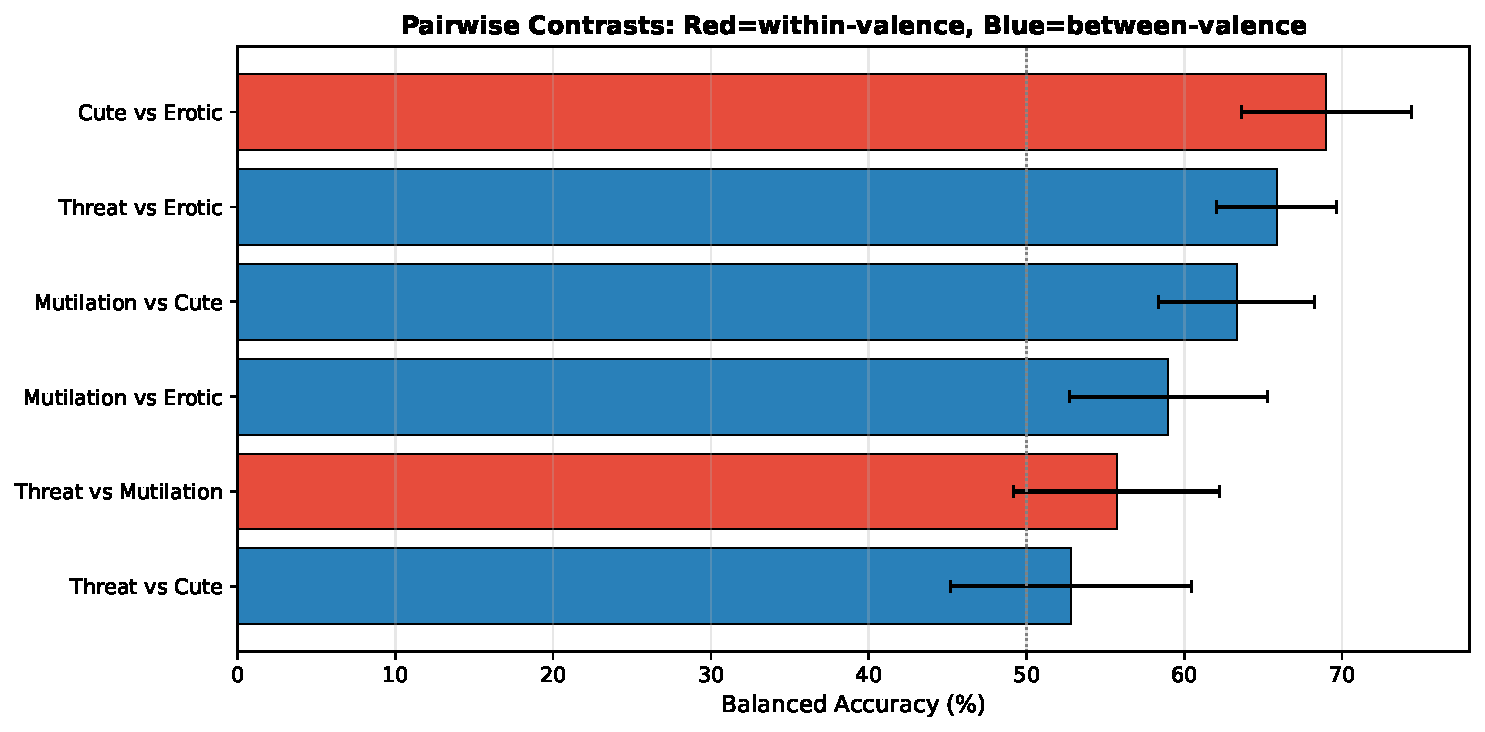
\includegraphics[width=\textwidth]{pictures/appendixA/ch5_4class_fig03_pairwise_contrasts.pdf}
    \caption{Pairwise classification accuracy hierarchy at four-class resolution. Cute vs.\ Erotic ($69.0\%$) is the easiest discrimination despite being within-valence; Threat vs.\ Cute ($52.8\%$) is the hardest despite being between-valence. This hierarchy tracks arousal rather than valence, indicating the reservoir's driven trajectory is more sensitive to the arousal dimension of affective input.}
    \label{fig:app_4class_fig03}
\end{figure}

\begin{figure}[H]
    \centering
    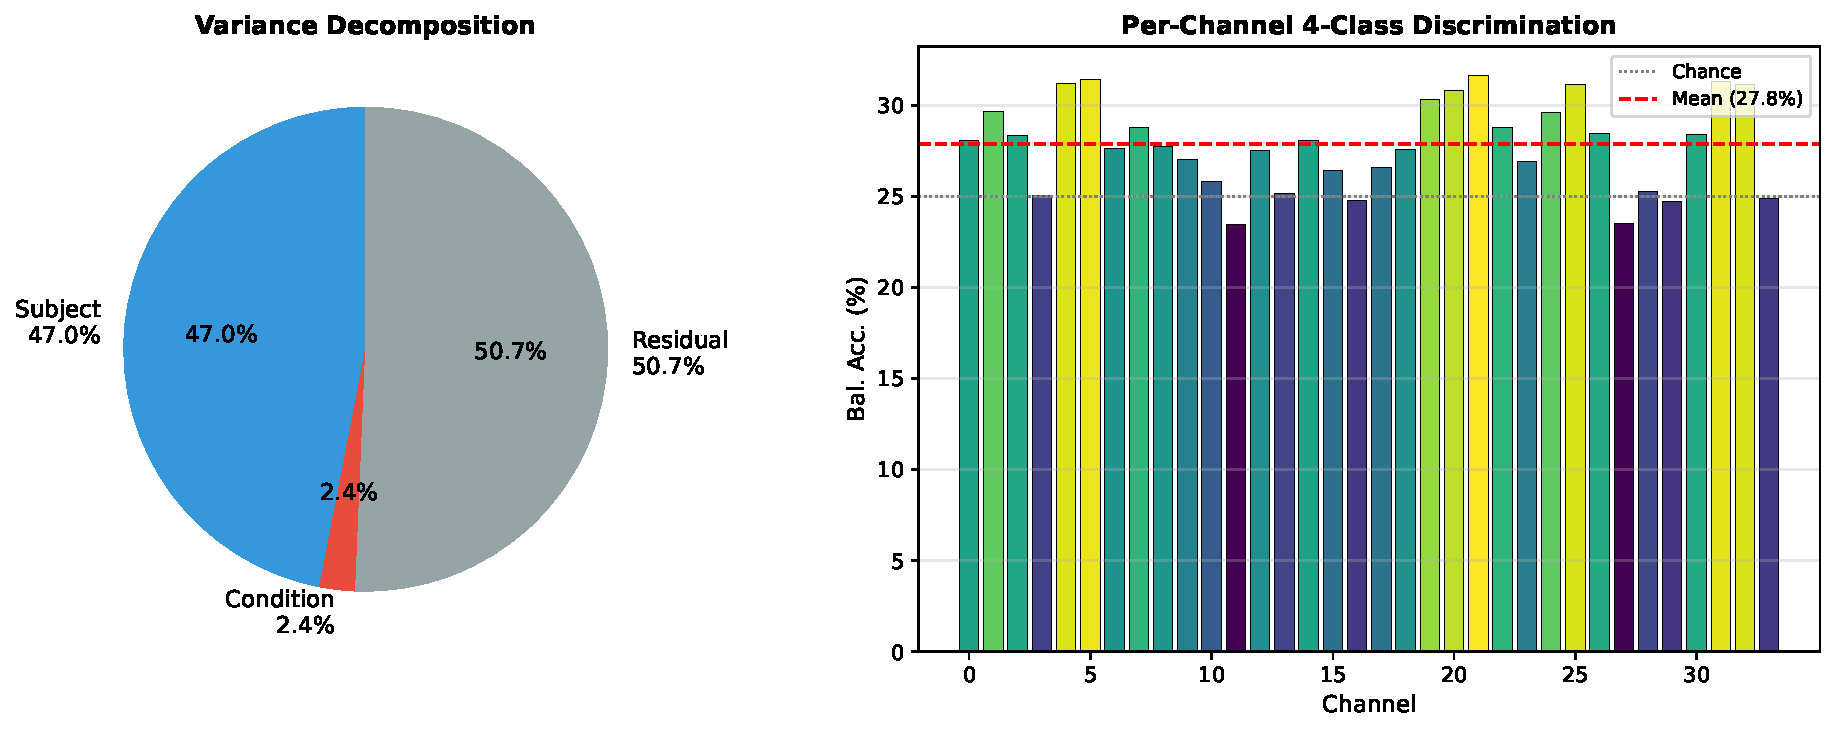
\includegraphics[width=\textwidth]{pictures/appendixA/ch5_4class_fig04_variance_channels.pdf}
    \caption{Variance decomposition and per-channel analysis at four-class resolution. Subject identity accounts for $47.0\%$ of embedding variance (vs.\ $62.6\%$ at three-class), condition accounts for $2.4\%$ (vs.\ $8.7\%$), and residual accounts for $50.7\%$. The subject-to-condition ratio increases from $7.2\times$ to $19.6\times$.}
    \label{fig:app_4class_fig04}
\end{figure}

\begin{figure}[H]
    \centering
    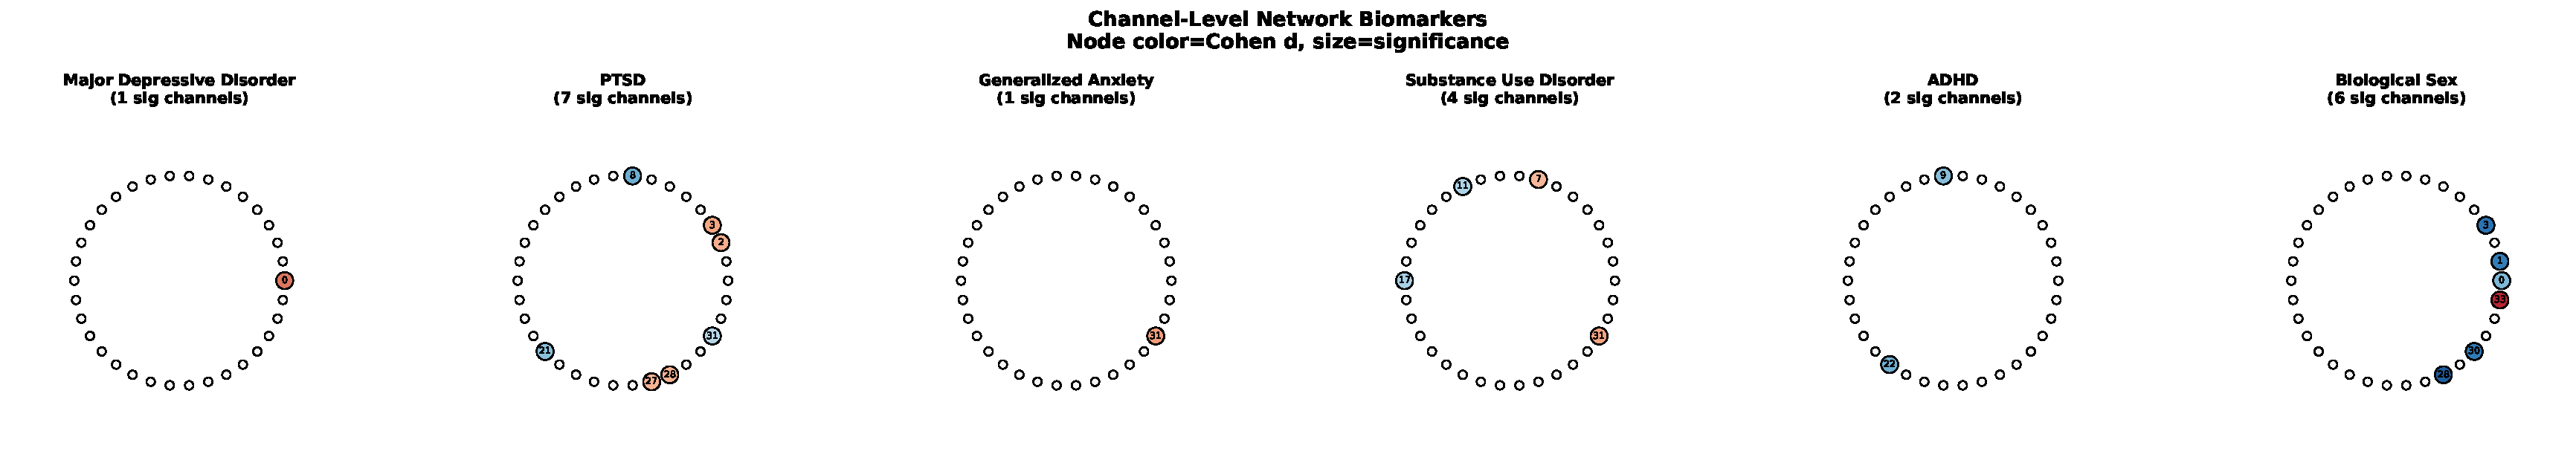
\includegraphics[width=\textwidth]{pictures/appendixA/ch5_4class_fig05_channel_biomarkers.pdf}
    \caption{Channel-level clinical biomarkers at four-class resolution. PTSD dominates with $11$ significant channel-metric pairs (vs.\ $6$ at three-class), displacing SUD as the primary clinical variable. The channel distribution of PTSD effects differs from the SUD distribution observed at three-class, indicating that different disorders produce spatially distinct network signatures.}
    \label{fig:app_4class_fig05}
\end{figure}

\begin{figure}[H]
    \centering
    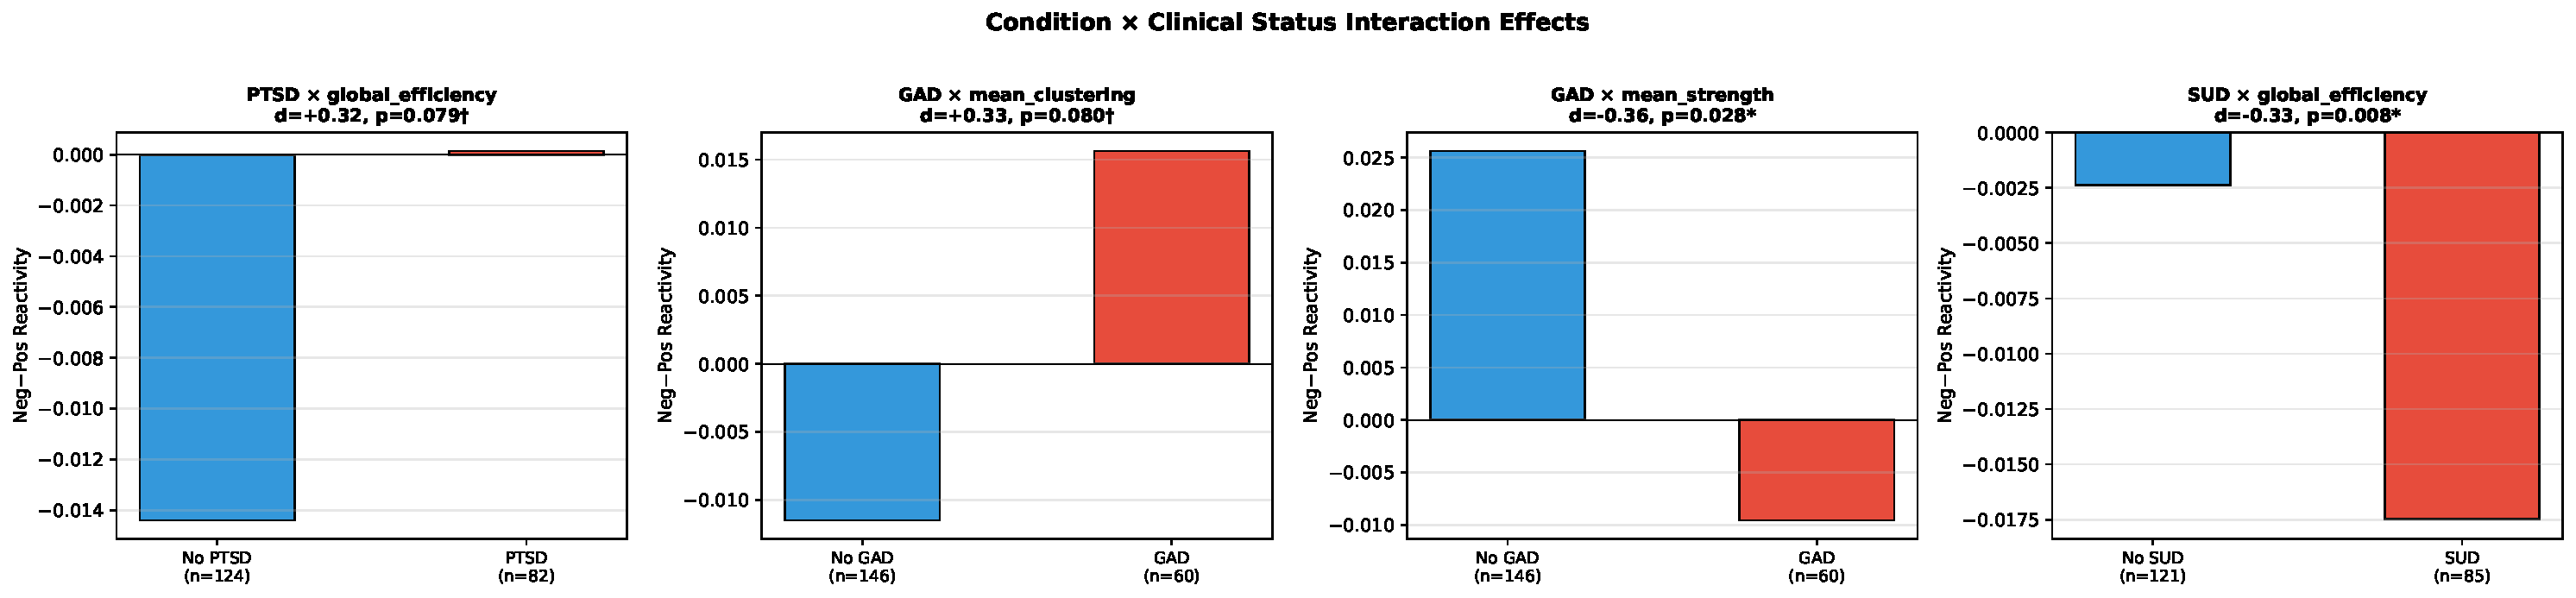
\includegraphics[width=\textwidth]{pictures/appendixA/ch5_4class_fig06_interactions.pdf}
    \caption{Condition $\times$ clinical interactions at four-class resolution. The PTSD $\times$ Threat--Mutilation interaction ($p = 0.036$) is the signature finding: PTSD subjects show differential network reorganization to threat-relevant versus general aversive stimuli. This interaction is structurally impossible at three-class, where both threat and mutilation images are collapsed into the Negative condition. The SUD $\times$ global efficiency interaction replicates from three-class ($p = 0.008$).}
    \label{fig:app_4class_fig06}
\end{figure}

\begin{figure}[H]
    \centering
    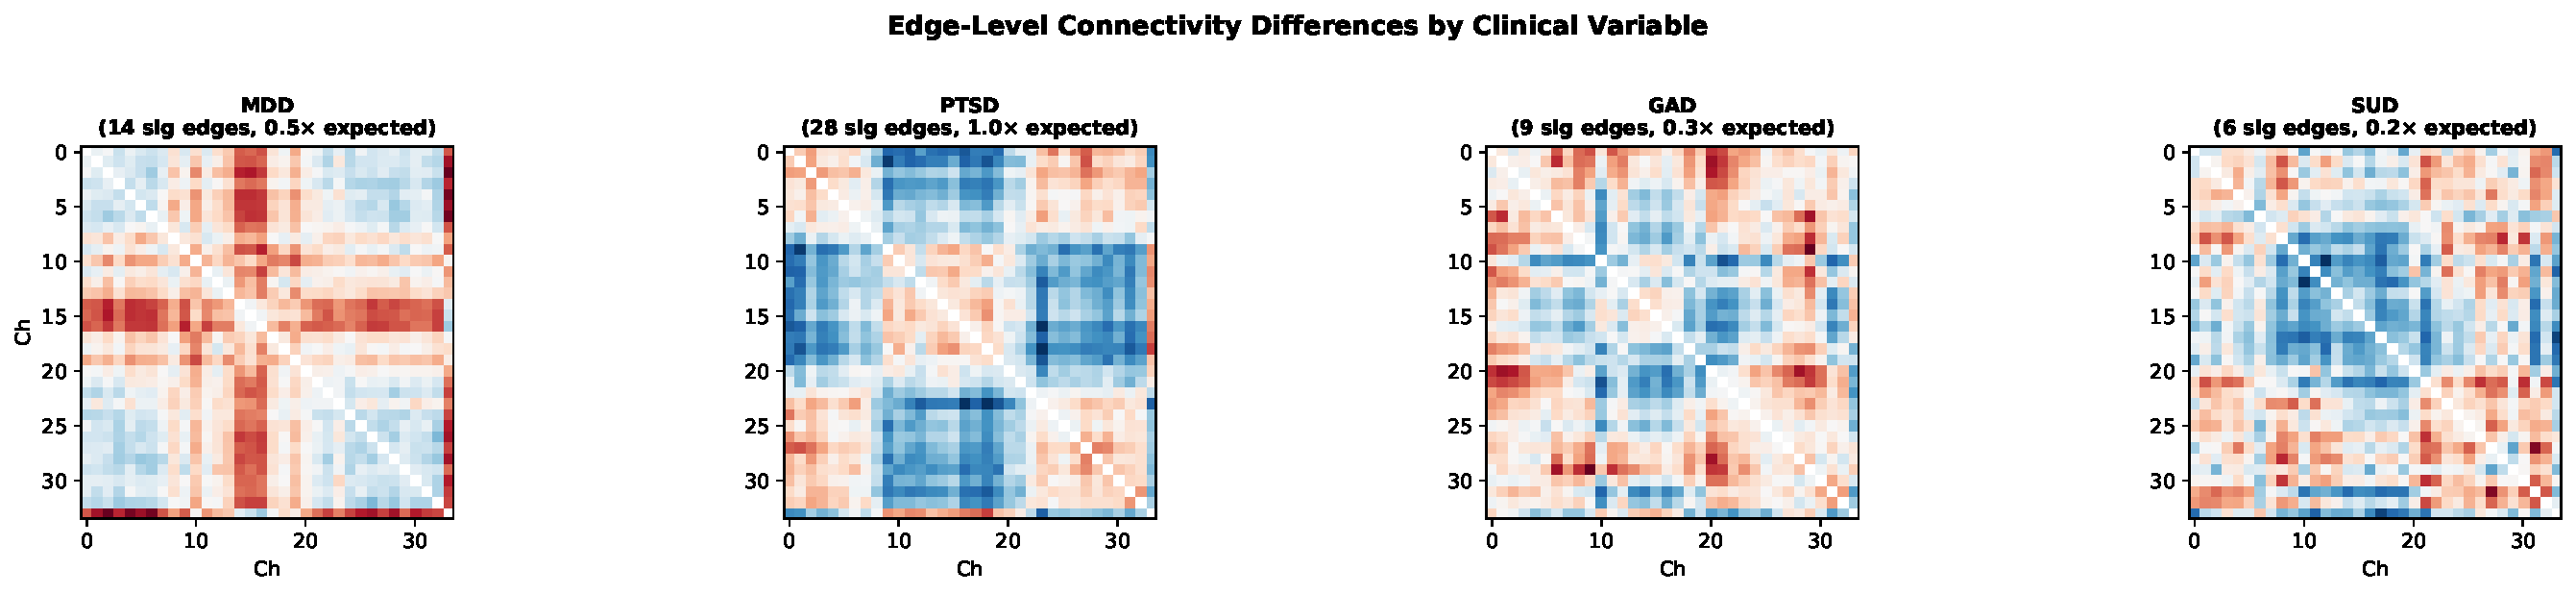
\includegraphics[width=\textwidth]{pictures/appendixA/ch5_4class_fig07_edge_biomarkers.pdf}
    \caption{Edge-level biomarkers at four-class resolution. PTSD produces $28$ significant edges (vs.\ $0$ surviving FDR correction at three-class). The finer affective resolution reveals edge-level clinical structure that the coarser three-class grouping obscures.}
    \label{fig:app_4class_fig07}
\end{figure}

\begin{figure}[H]
    \centering
    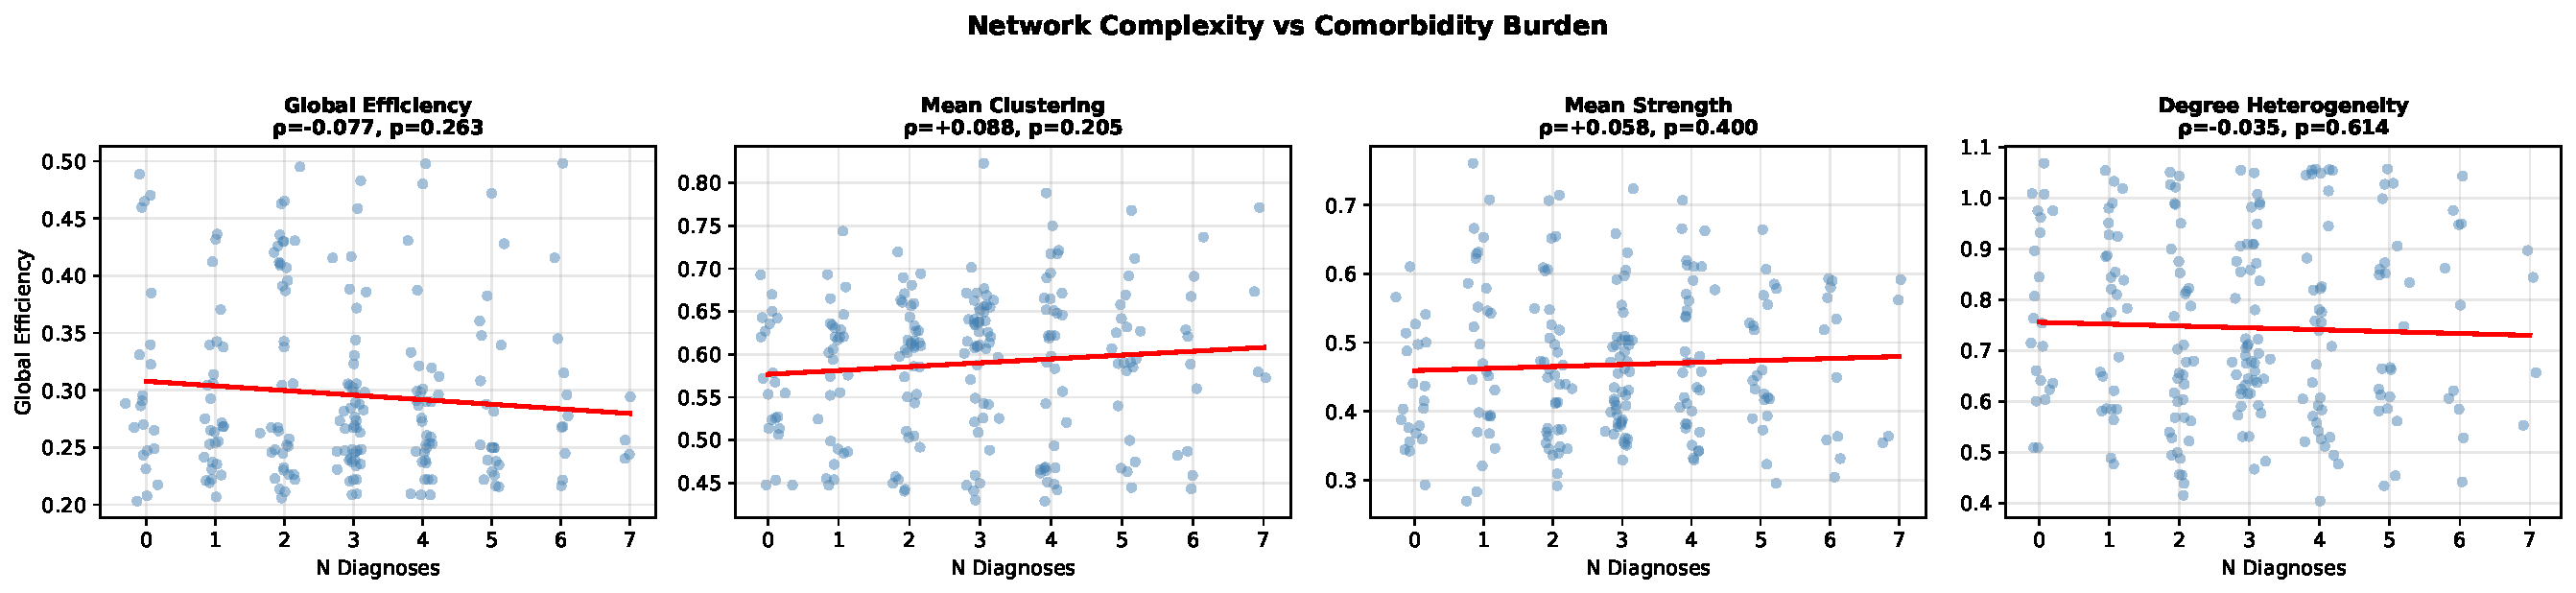
\includegraphics[width=\textwidth]{pictures/appendixA/ch5_4class_fig08_comorbidity.pdf}
    \caption{Comorbidity analysis at four-class resolution. Comorbidity count does not significantly correlate with any graph-level network metric, indicating that the disorder-specific findings (PTSD, SUD) are not driven by general psychiatric burden.}
    \label{fig:app_4class_fig08}
\end{figure}

\begin{figure}[H]
    \centering
    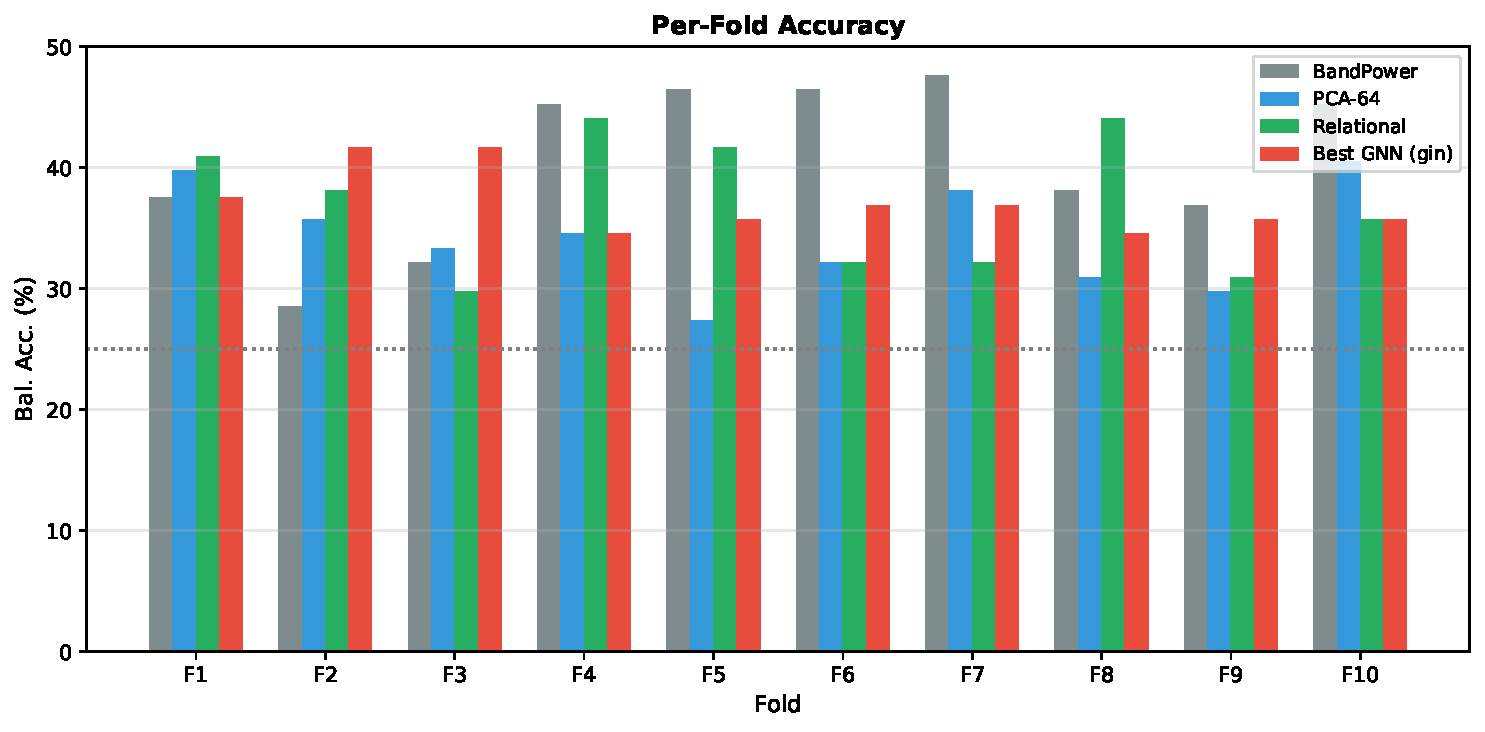
\includegraphics[width=\textwidth]{pictures/appendixA/ch5_4class_fig09_fold_comparison.pdf}
    \caption{Cross-fold stability at four-class resolution. Per-fold accuracy distributions for band-power, reservoir, and GNN classifiers. The band-power advantage over the reservoir is consistent across folds, confirming that the regime inversion is robust.}
    \label{fig:app_4class_fig09}
\end{figure}


%% ═══════════════════════════════════════════════════════════════
%% SECTION A.3: LAYER ABLATION FIGURES
%% ═══════════════════════════════════════════════════════════════
\section{Layer Ablation and Complementarity Figures}
\label{app:ablation}

The following three figures present the complete visualization of the layer ablation experiment reported in Chapter~\ref{chap:arspi_net}, Section~\ref{sec:ch5_ablation}. The numerical results are presented in Tables~\ref{tab:emotion_ablation} and~\ref{tab:clinical_ablation} in the main text.

\begin{figure}[H]
    \centering
    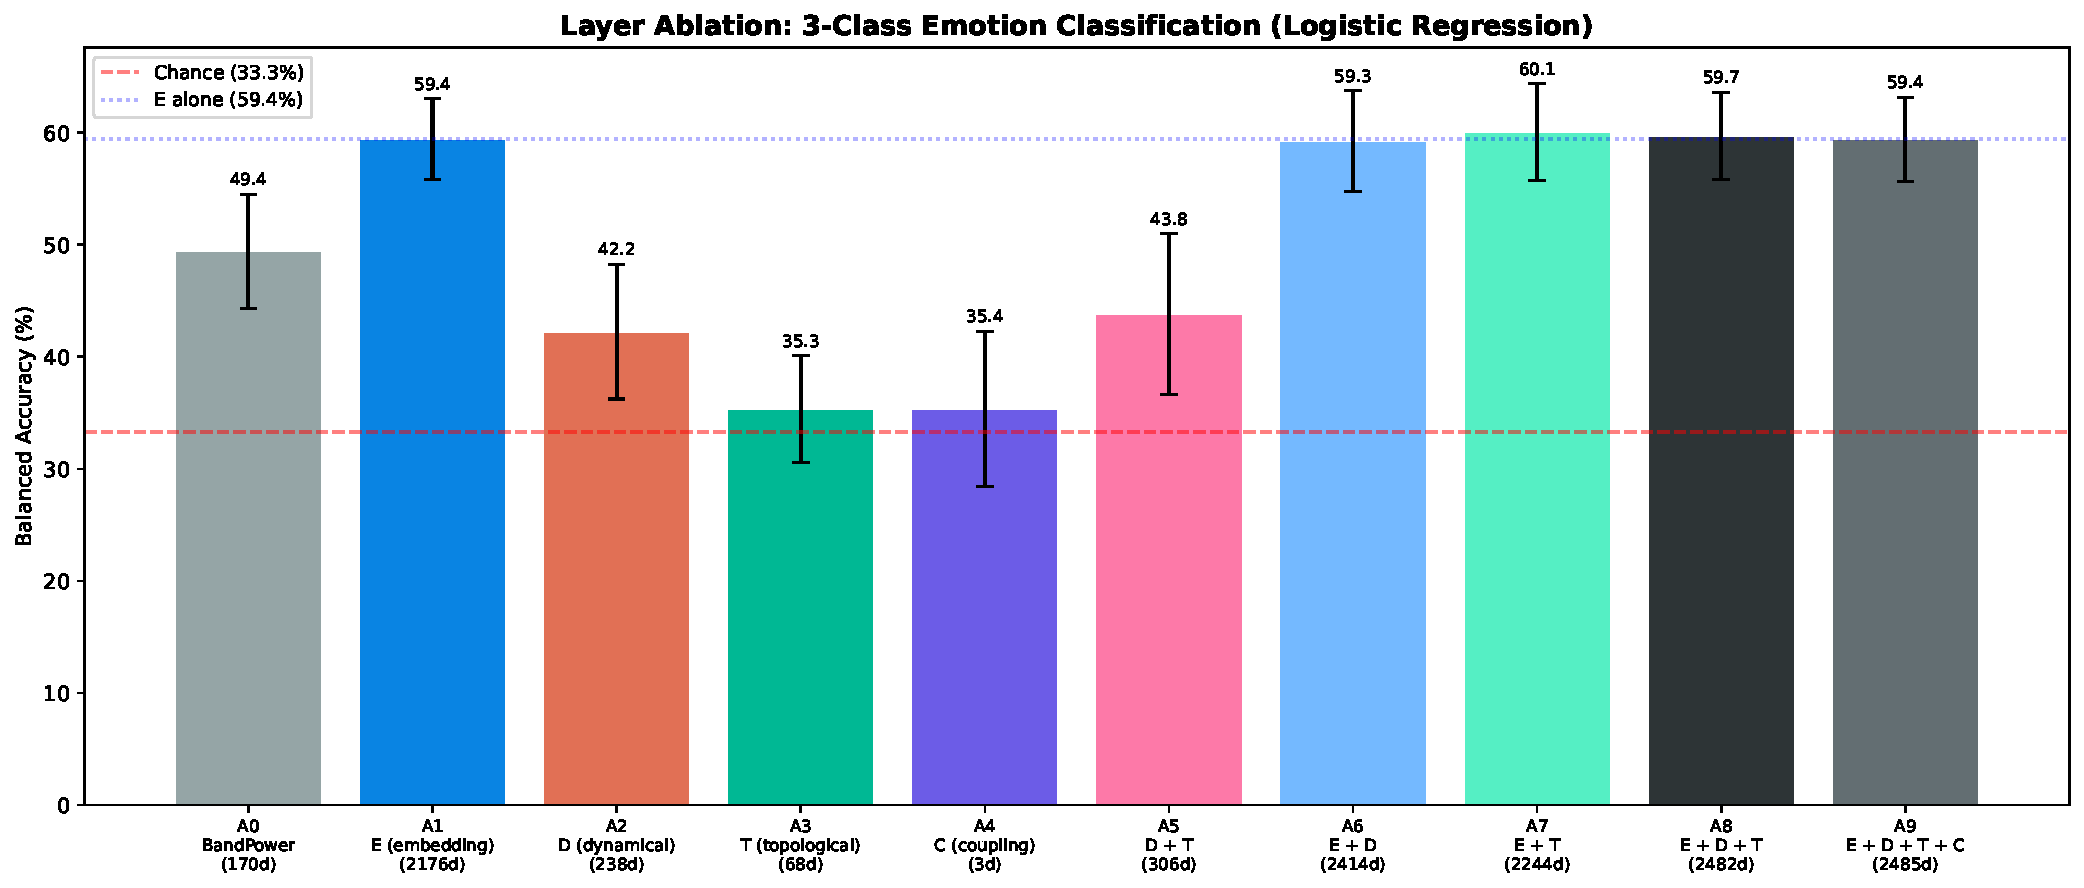
\includegraphics[width=\textwidth]{pictures/appendixA/ch5_fig_emotion_ablation.pdf}
    \caption{Layer ablation: three-class emotion classification (logistic regression, $10$-fold subject-level CV). A0: band-power ($49.4\%$). A1: embedding alone ($59.4\%$). A2: dynamical metrics ($42.2\%$). A3: topological metrics ($35.3\%$). A4: coupling ($35.4\%$). A5--A9: combinations. The embedding (A1) is the primary discriminative substrate; no combination exceeds it by more than $0.7$~pp. Error bars: standard deviation across folds.}
    \label{fig:app_emotion_ablation}
\end{figure}

\begin{figure}[H]
    \centering
    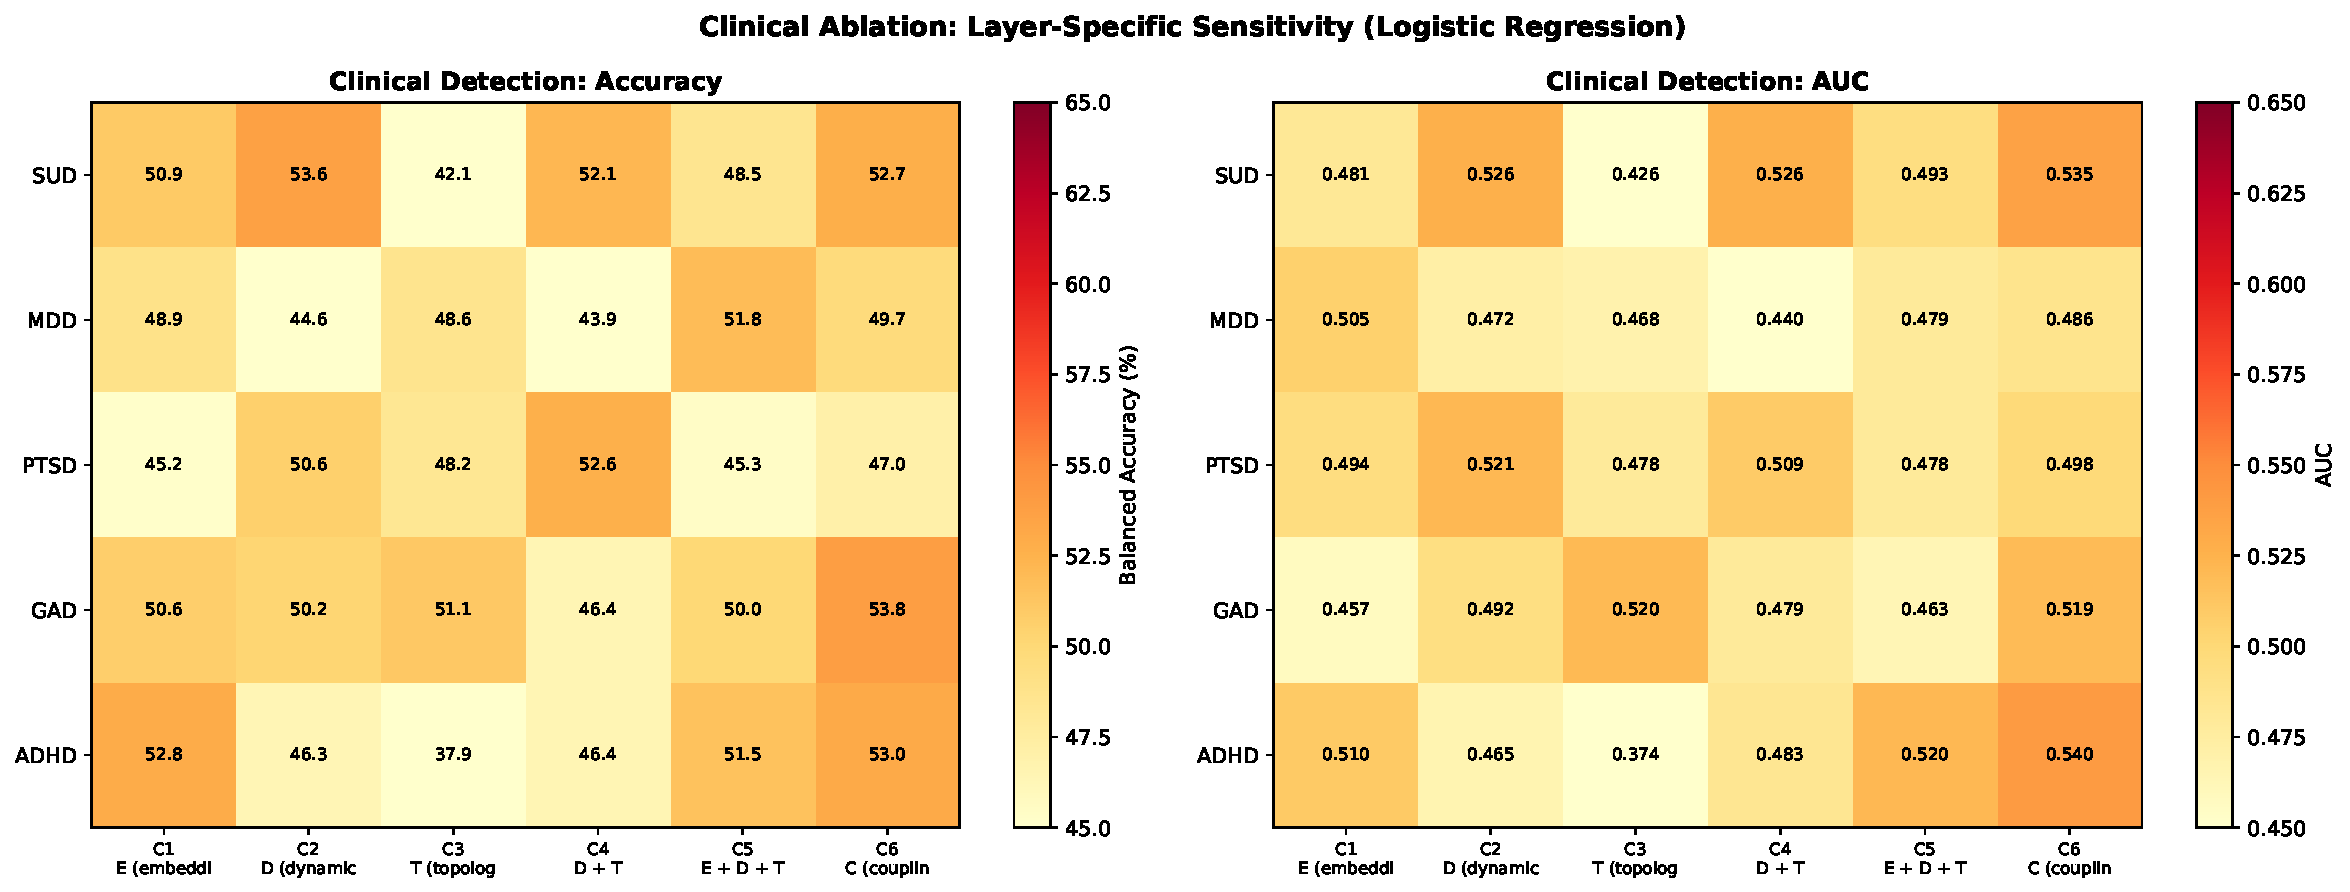
\includegraphics[width=\textwidth]{pictures/appendixA/ch5_fig_clinical_ablation.pdf}
    \caption{Clinical detection ablation (logistic regression, $5$-fold subject-level CV). Left: balanced accuracy by feature block and disorder. Right: AUC by feature block and disorder. The strongest layer differs across diagnoses: dynamics (C2) for SUD and PTSD, topology (C3) for GAD, coupling (C6) for ADHD. This layer-specific sensitivity pattern supports the interpretation that ARSPI-Net's three response layers are operationally distinct.}
    \label{fig:app_clinical_ablation}
\end{figure}

\begin{figure}[H]
    \centering
    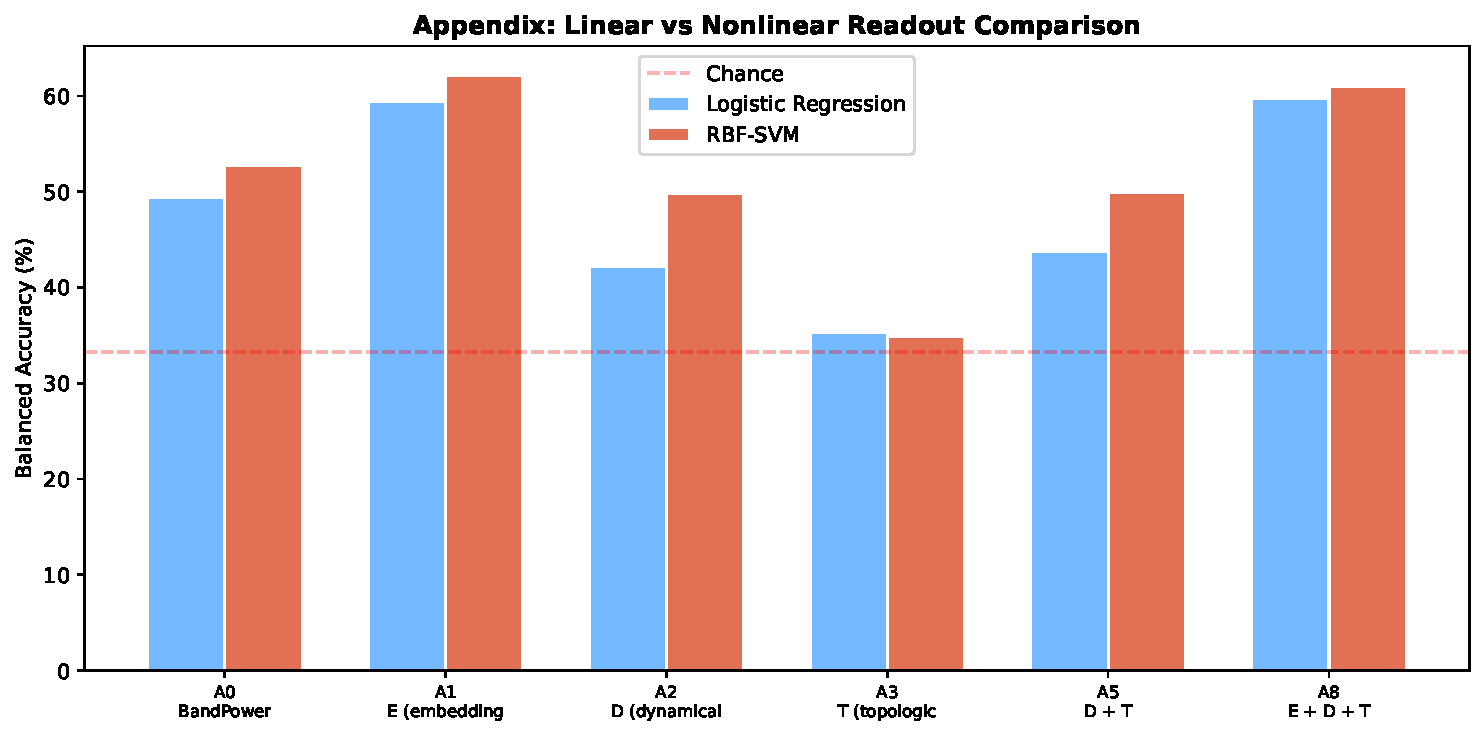
\includegraphics[width=\textwidth]{pictures/appendixA/ch5_fig_rbf_sensitivity.pdf}
    \caption{Appendix sensitivity check: linear (logistic regression) versus nonlinear (RBF-SVM) readout comparison for selected feature blocks. The embedding (A1) rises from $59.4\%$ to $62.1\%$ under nonlinear readout. Dynamical metrics (A2) benefit most ($+7.5$~pp, from $42.2\%$ to $49.8\%$), indicating their condition information is not linearly separable but partially recoverable by a nonlinear classifier. The ranking structure is preserved across readout choice.}
    \label{fig:app_rbf_sensitivity}
\end{figure}


%% ═══════════════════════════════════════════════════════════════
%% SECTION A.4: CHAPTER 6 FIGURES
%% ═══════════════════════════════════════════════════════════════
\section{Chapter 6: Supplementary Raw Observations}
\label{app:ch6_figs}

The following eight observation figures characterize the dynamical and topological features extracted from the SHAPE dataset prior to the experimental analyses reported in Chapter~\ref{chap:dynamics}. They establish metric distributions, channel heterogeneity, population firing rate temporal structure, connectivity patterns, and clinical metadata coverage. The seven experimental result figures (EXP-6.1 through EXP-6.7) are presented inline in Chapter~\ref{chap:dynamics}.

\begin{figure}[H]
    \centering
    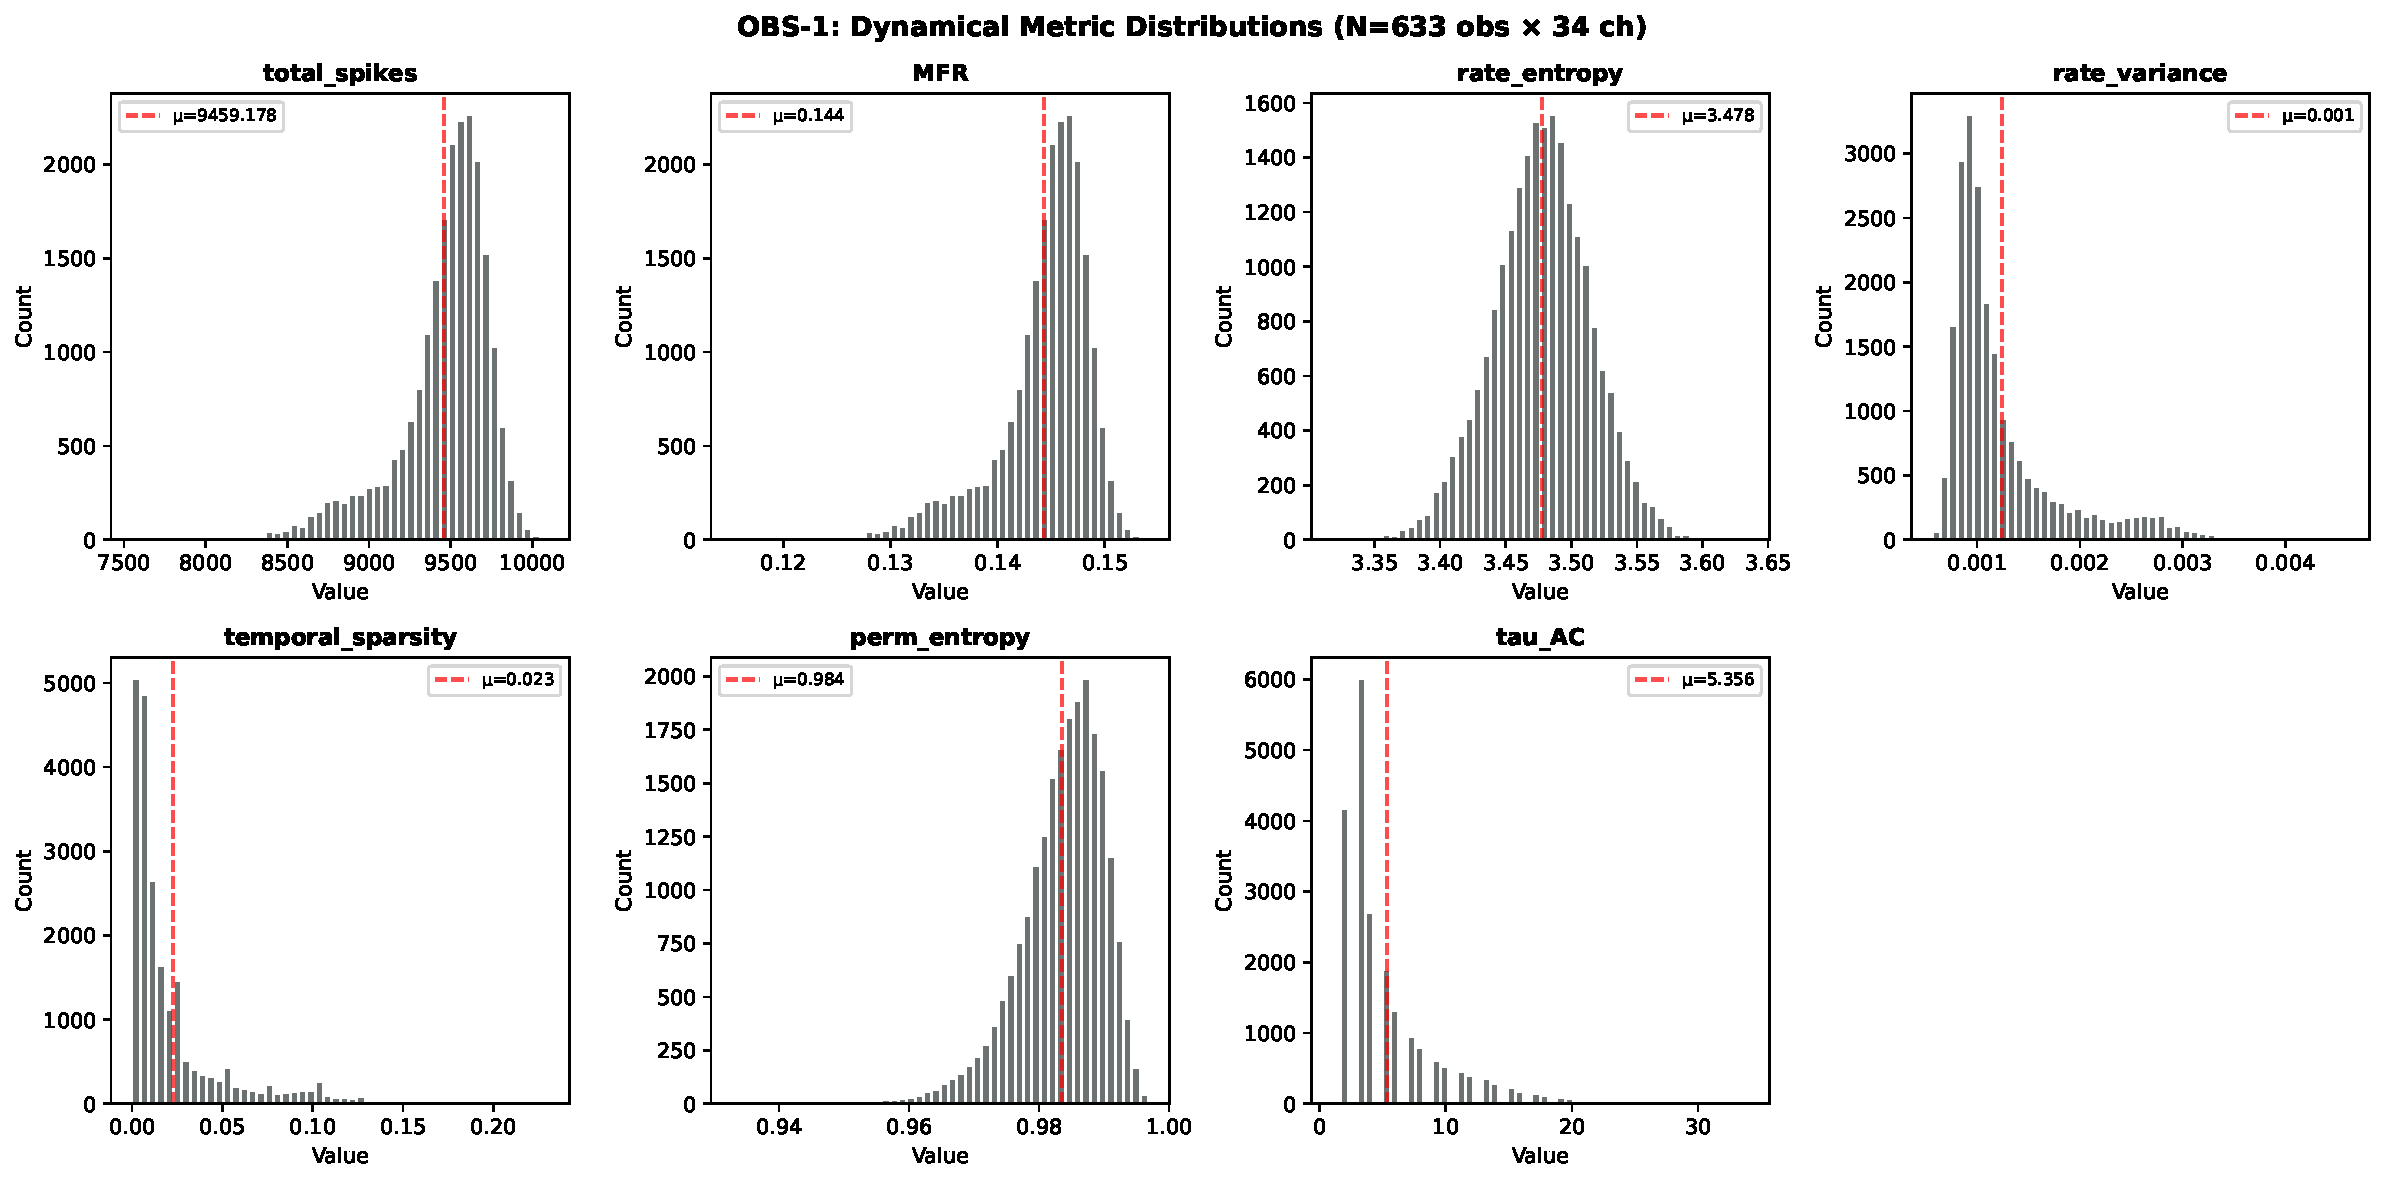
\includegraphics[width=\textwidth]{pictures/appendixA/obs01_metric_distributions.pdf}
    \caption{OBS-1: Dynamical metric distributions across all $633$ observations ($211$ subjects $\times$ $3$ conditions). Seven core metrics span different variability regimes: $\tau_{\text{AC}}$ (CV~$= 0.77$) and temporal sparsity (CV~$= 1.24$) show the highest variability; MFR (CV~$= 0.03$) and permutation entropy (CV~$= 0.007$) show the lowest.}
    \label{fig:app_ch6_obs01}
\end{figure}

\begin{figure}[H]
    \centering
    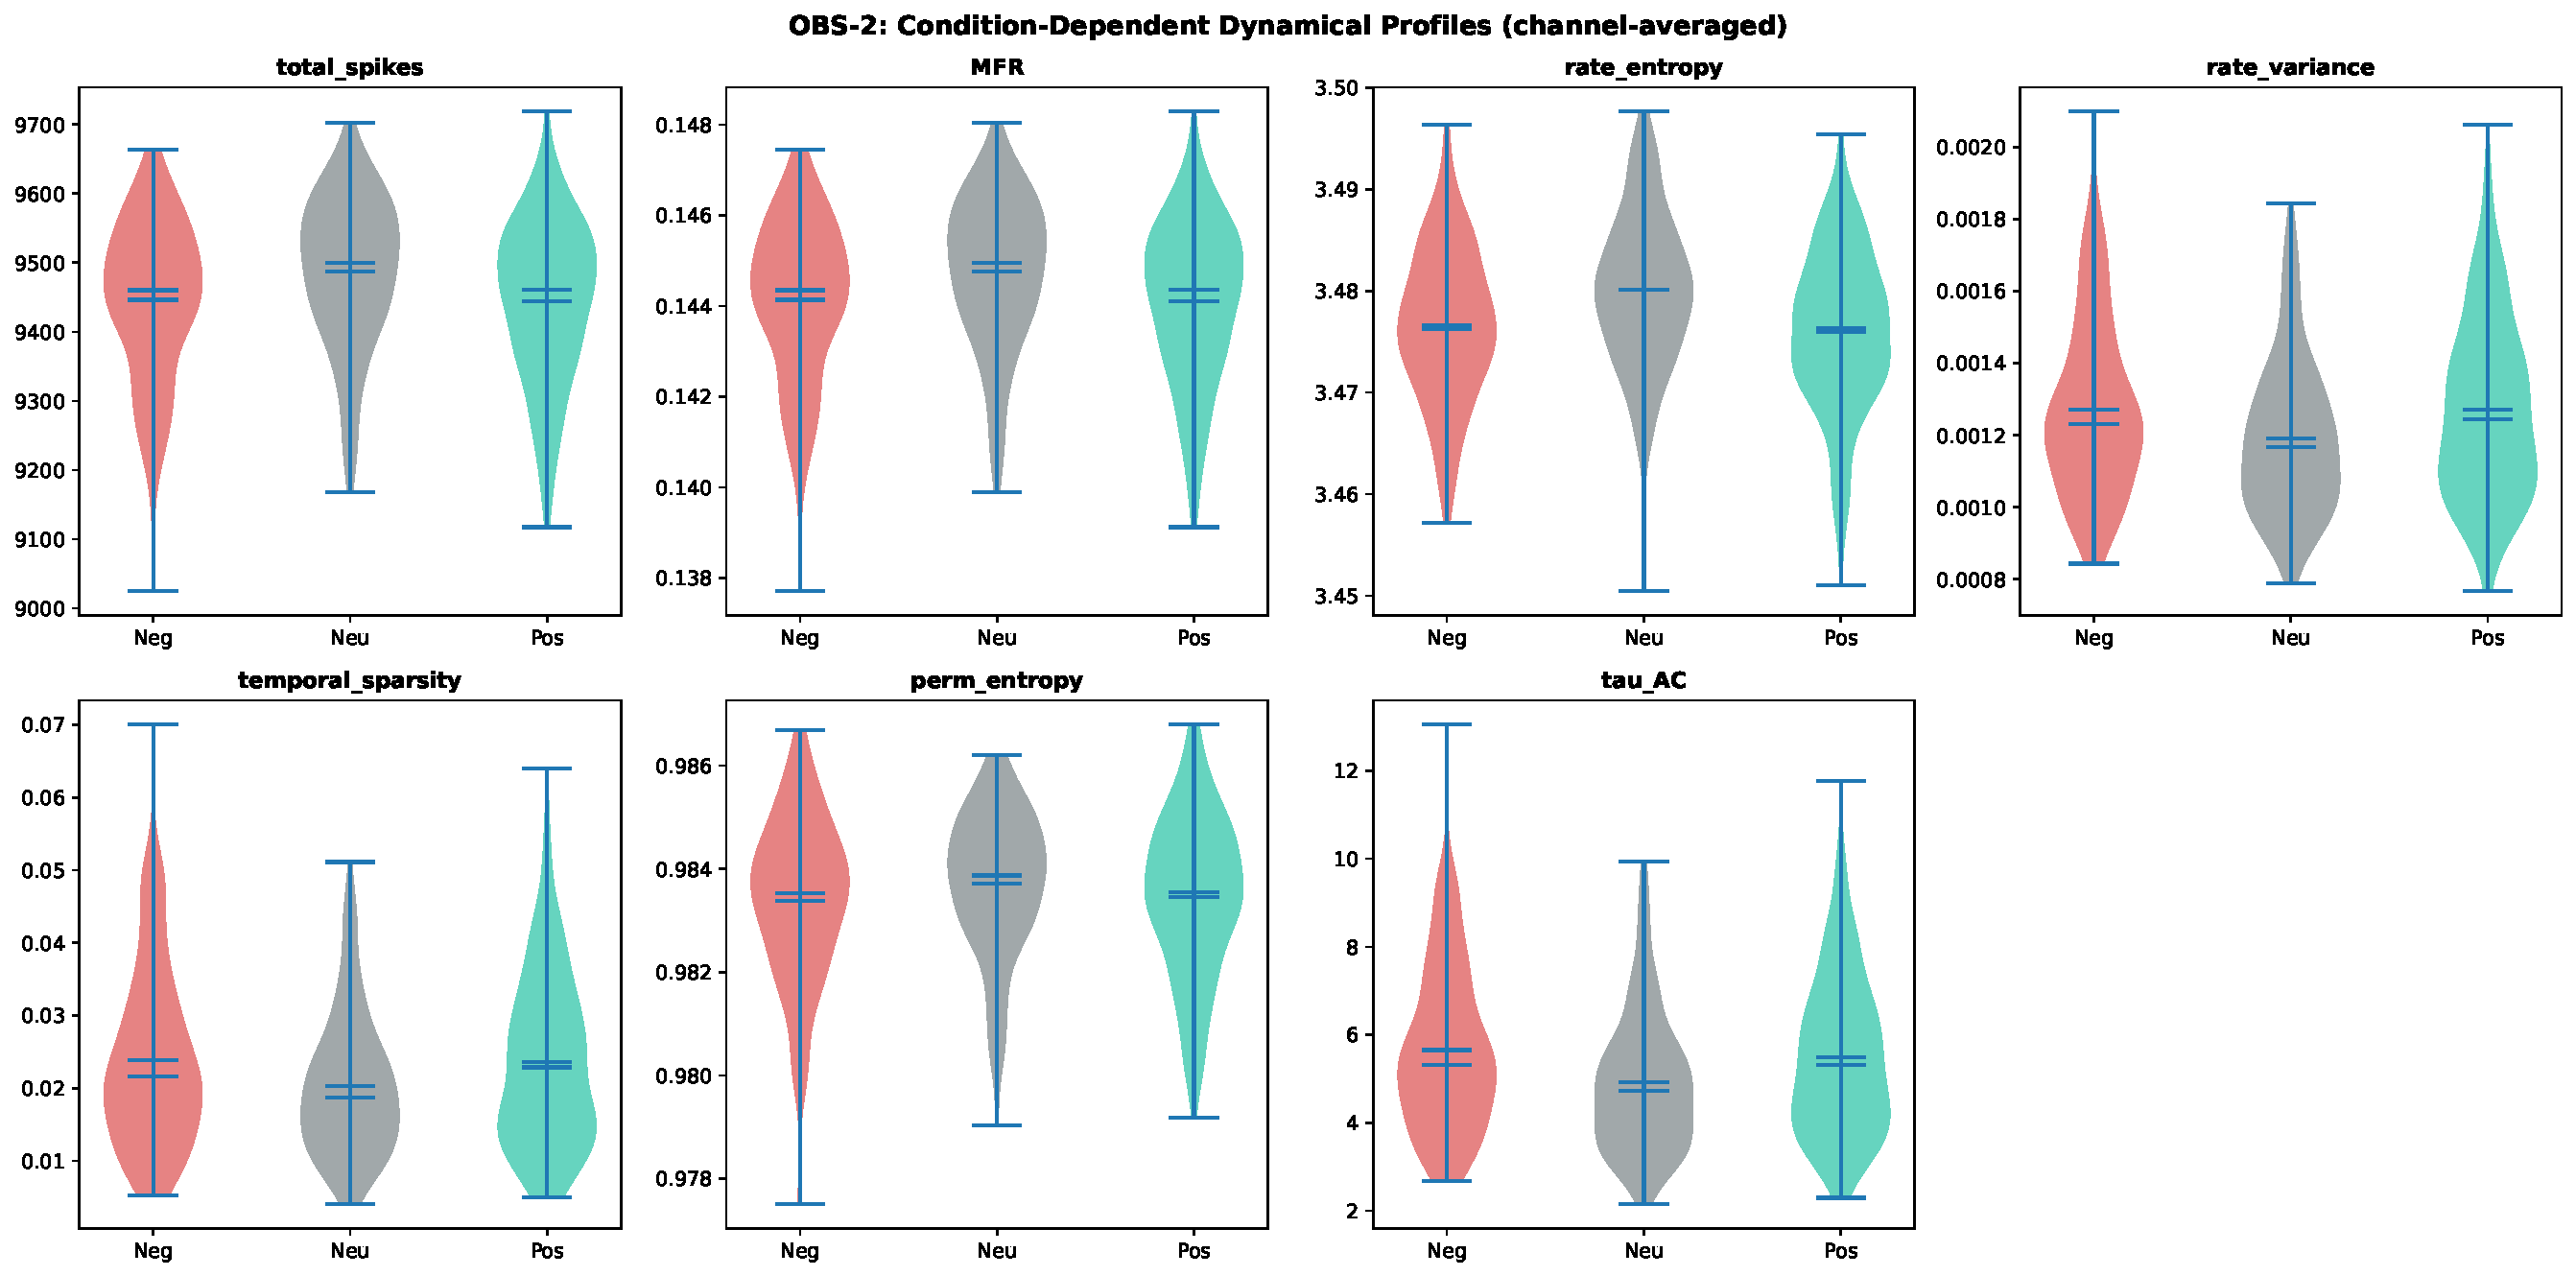
\includegraphics[width=\textwidth]{pictures/appendixA/obs02_condition_profiles.pdf}
    \caption{OBS-2: Condition-dependent dynamical profiles. Negative and Pleasant produce nearly identical values for all metrics, while Neutral is the outlier. The largest condition effect is $\tau_{\text{AC}}$: Negative ($5.65$) $>$ Pleasant ($5.50$) $>$ Neutral ($4.92$). The reservoir's dynamics track arousal rather than valence.}
    \label{fig:app_ch6_obs02}
\end{figure}

\begin{figure}[H]
    \centering
    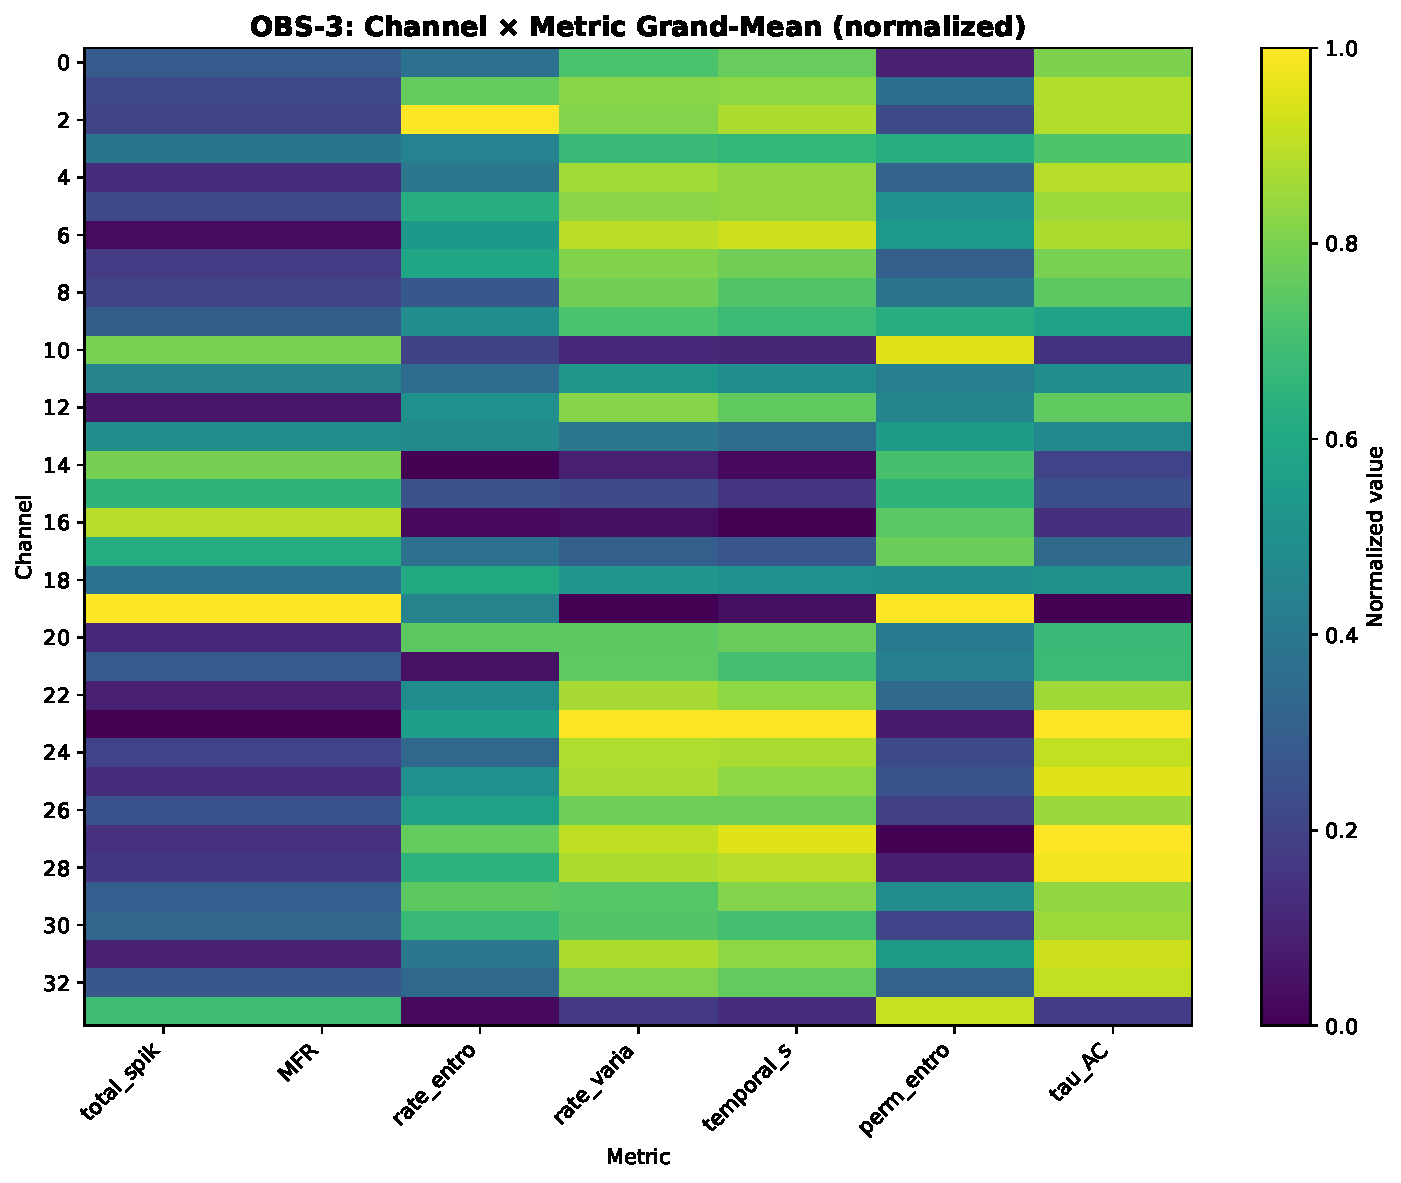
\includegraphics[width=\textwidth]{pictures/appendixA/obs03_channel_heterogeneity.pdf}
    \caption{OBS-3: Per-channel dynamical metric heterogeneity. Temporal sparsity ($2.54\times$ ratio between channels) and $\tau_{\text{AC}}$ ($1.56\times$) show the strongest channel gradients---the spatial structure that Chapter~\ref{chap:synthesis} exploits for coupling analysis. Rate entropy and permutation entropy are effectively constant across channels.}
    \label{fig:app_ch6_obs03}
\end{figure}

\begin{figure}[H]
    \centering
    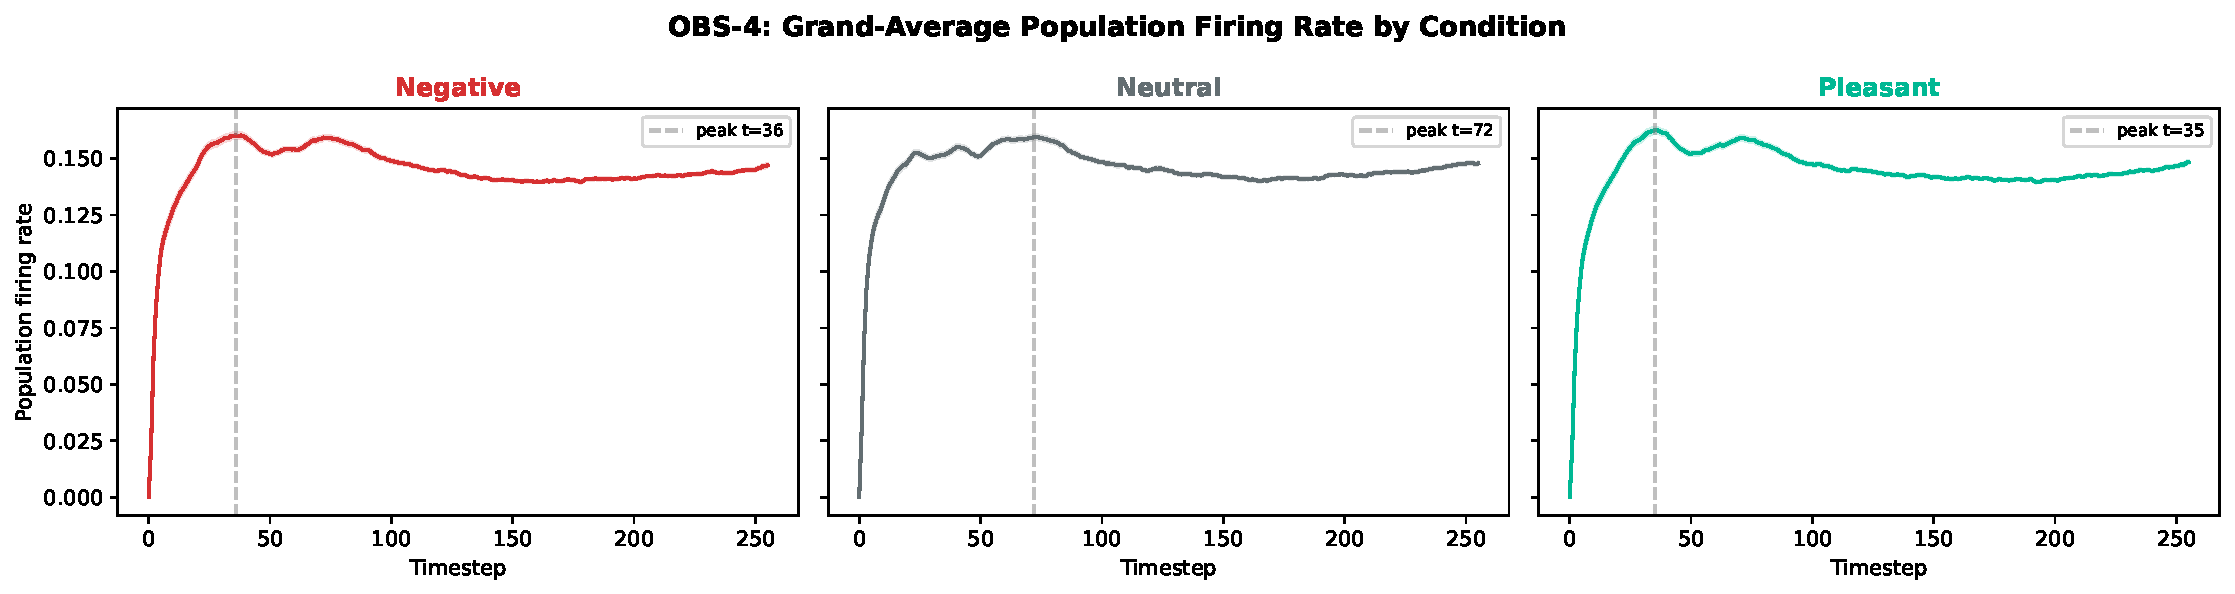
\includegraphics[width=\textwidth]{pictures/appendixA/obs04_firing_rate_timecourses.pdf}
    \caption{OBS-4: Grand-average population firing rate timecourses by condition. Negative and Pleasant peak at $t \approx 35$--$36$ (early); Neutral peaks at $t = 72$ (late). The $36$-timestep peak latency difference is a temporal signature of emotional salience. Peak-to-final ratio is largest for Pleasant ($1.11$).}
    \label{fig:app_ch6_obs04}
\end{figure}

\begin{figure}[H]
    \centering
    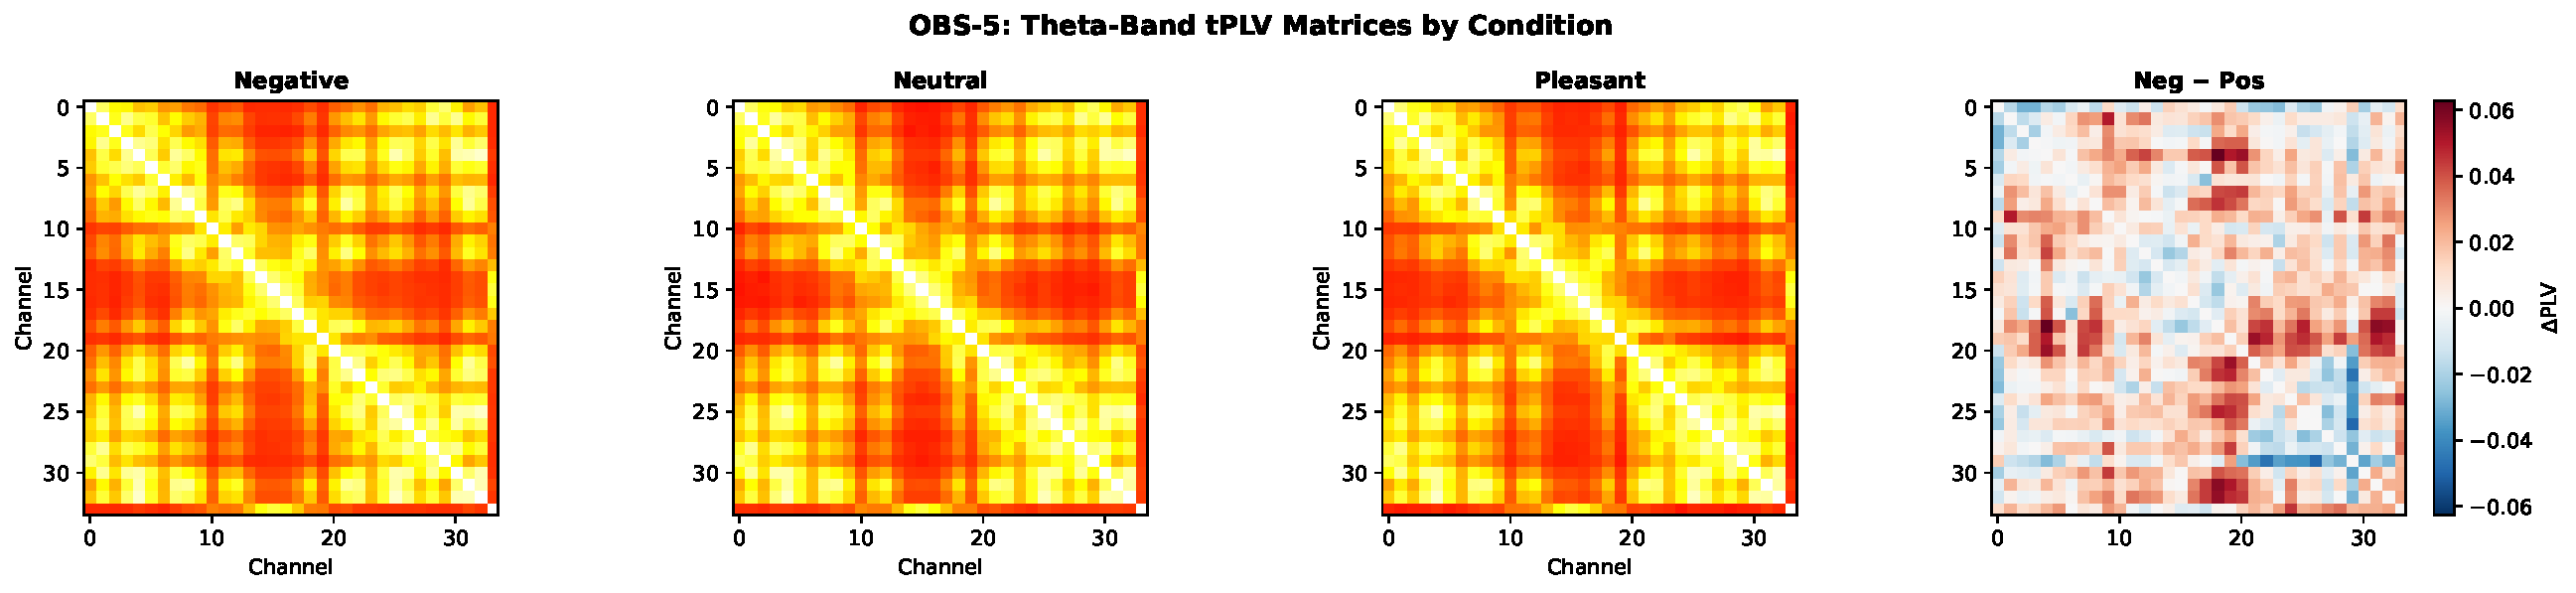
\includegraphics[width=\textwidth]{pictures/appendixA/obs05_tplv_connectivity.pdf}
    \caption{OBS-5: Theta-band phase-locking connectivity structure. Mean PLV is condition-dependent: Negative ($0.635$) $>$ Neutral ($0.632$) $>$ Pleasant ($0.626$). The largest pairwise contrast (Negative--Pleasant) has mean $|\Delta\text{PLV}| = 0.016$ and max $= 0.063$.}
    \label{fig:app_ch6_obs05}
\end{figure}

\begin{figure}[H]
    \centering
    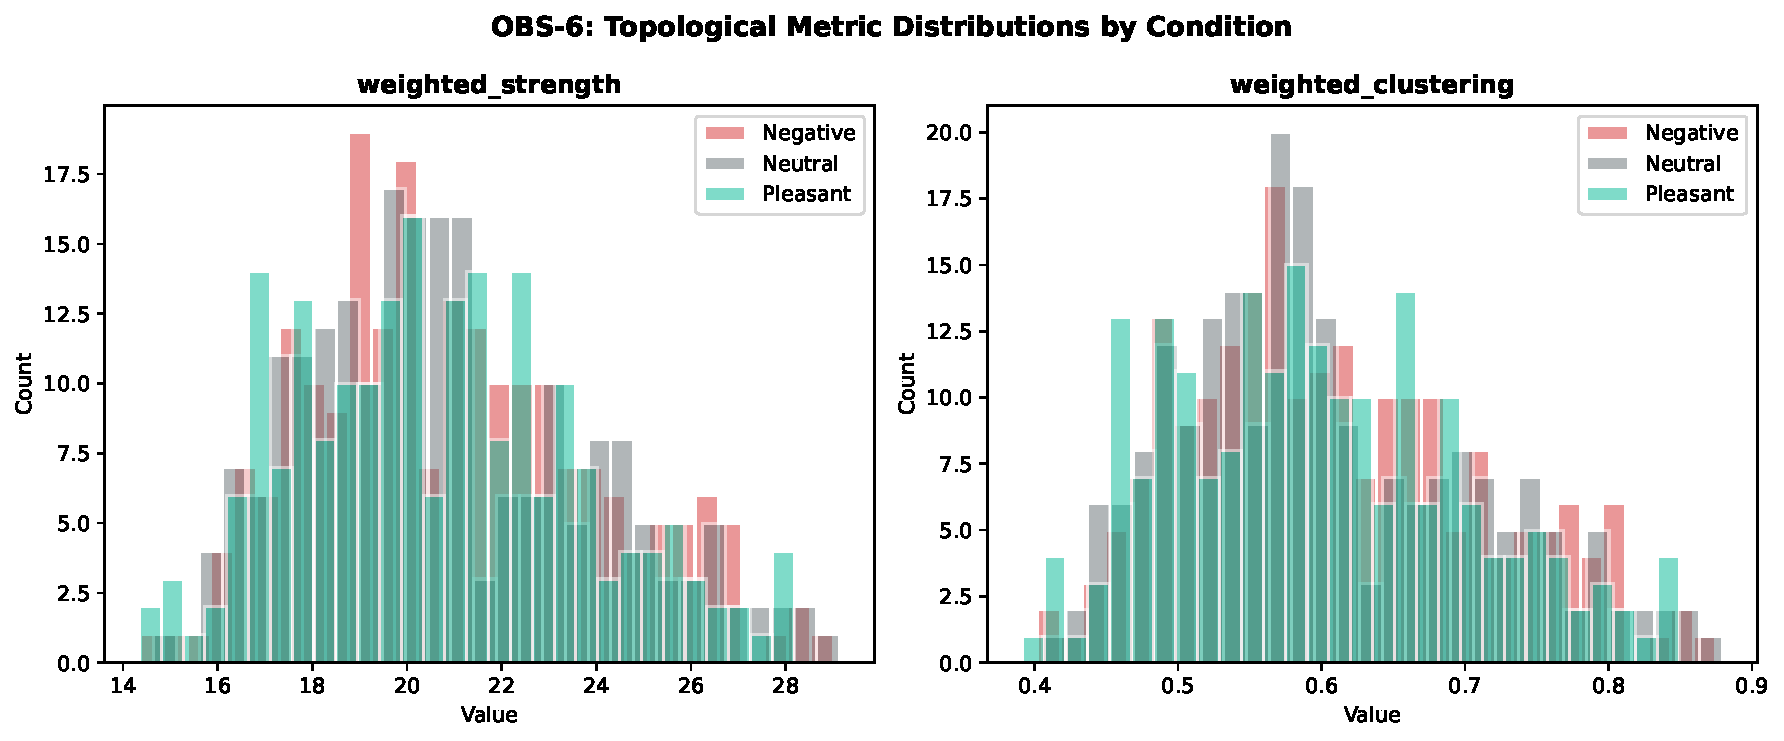
\includegraphics[width=\textwidth]{pictures/appendixA/obs06_topological_distributions.pdf}
    \caption{OBS-6: Topological metric distributions. Weighted node strength ranges from $5.9$ to $30.8$ ($5.2\times$ ratio); weighted clustering ranges from $0.21$ to $0.91$. Both show Negative $>$ Neutral $>$ Pleasant ordering. The wide per-channel ranges provide the spatial heterogeneity required for coupling analysis.}
    \label{fig:app_ch6_obs06}
\end{figure}

\begin{figure}[H]
    \centering
    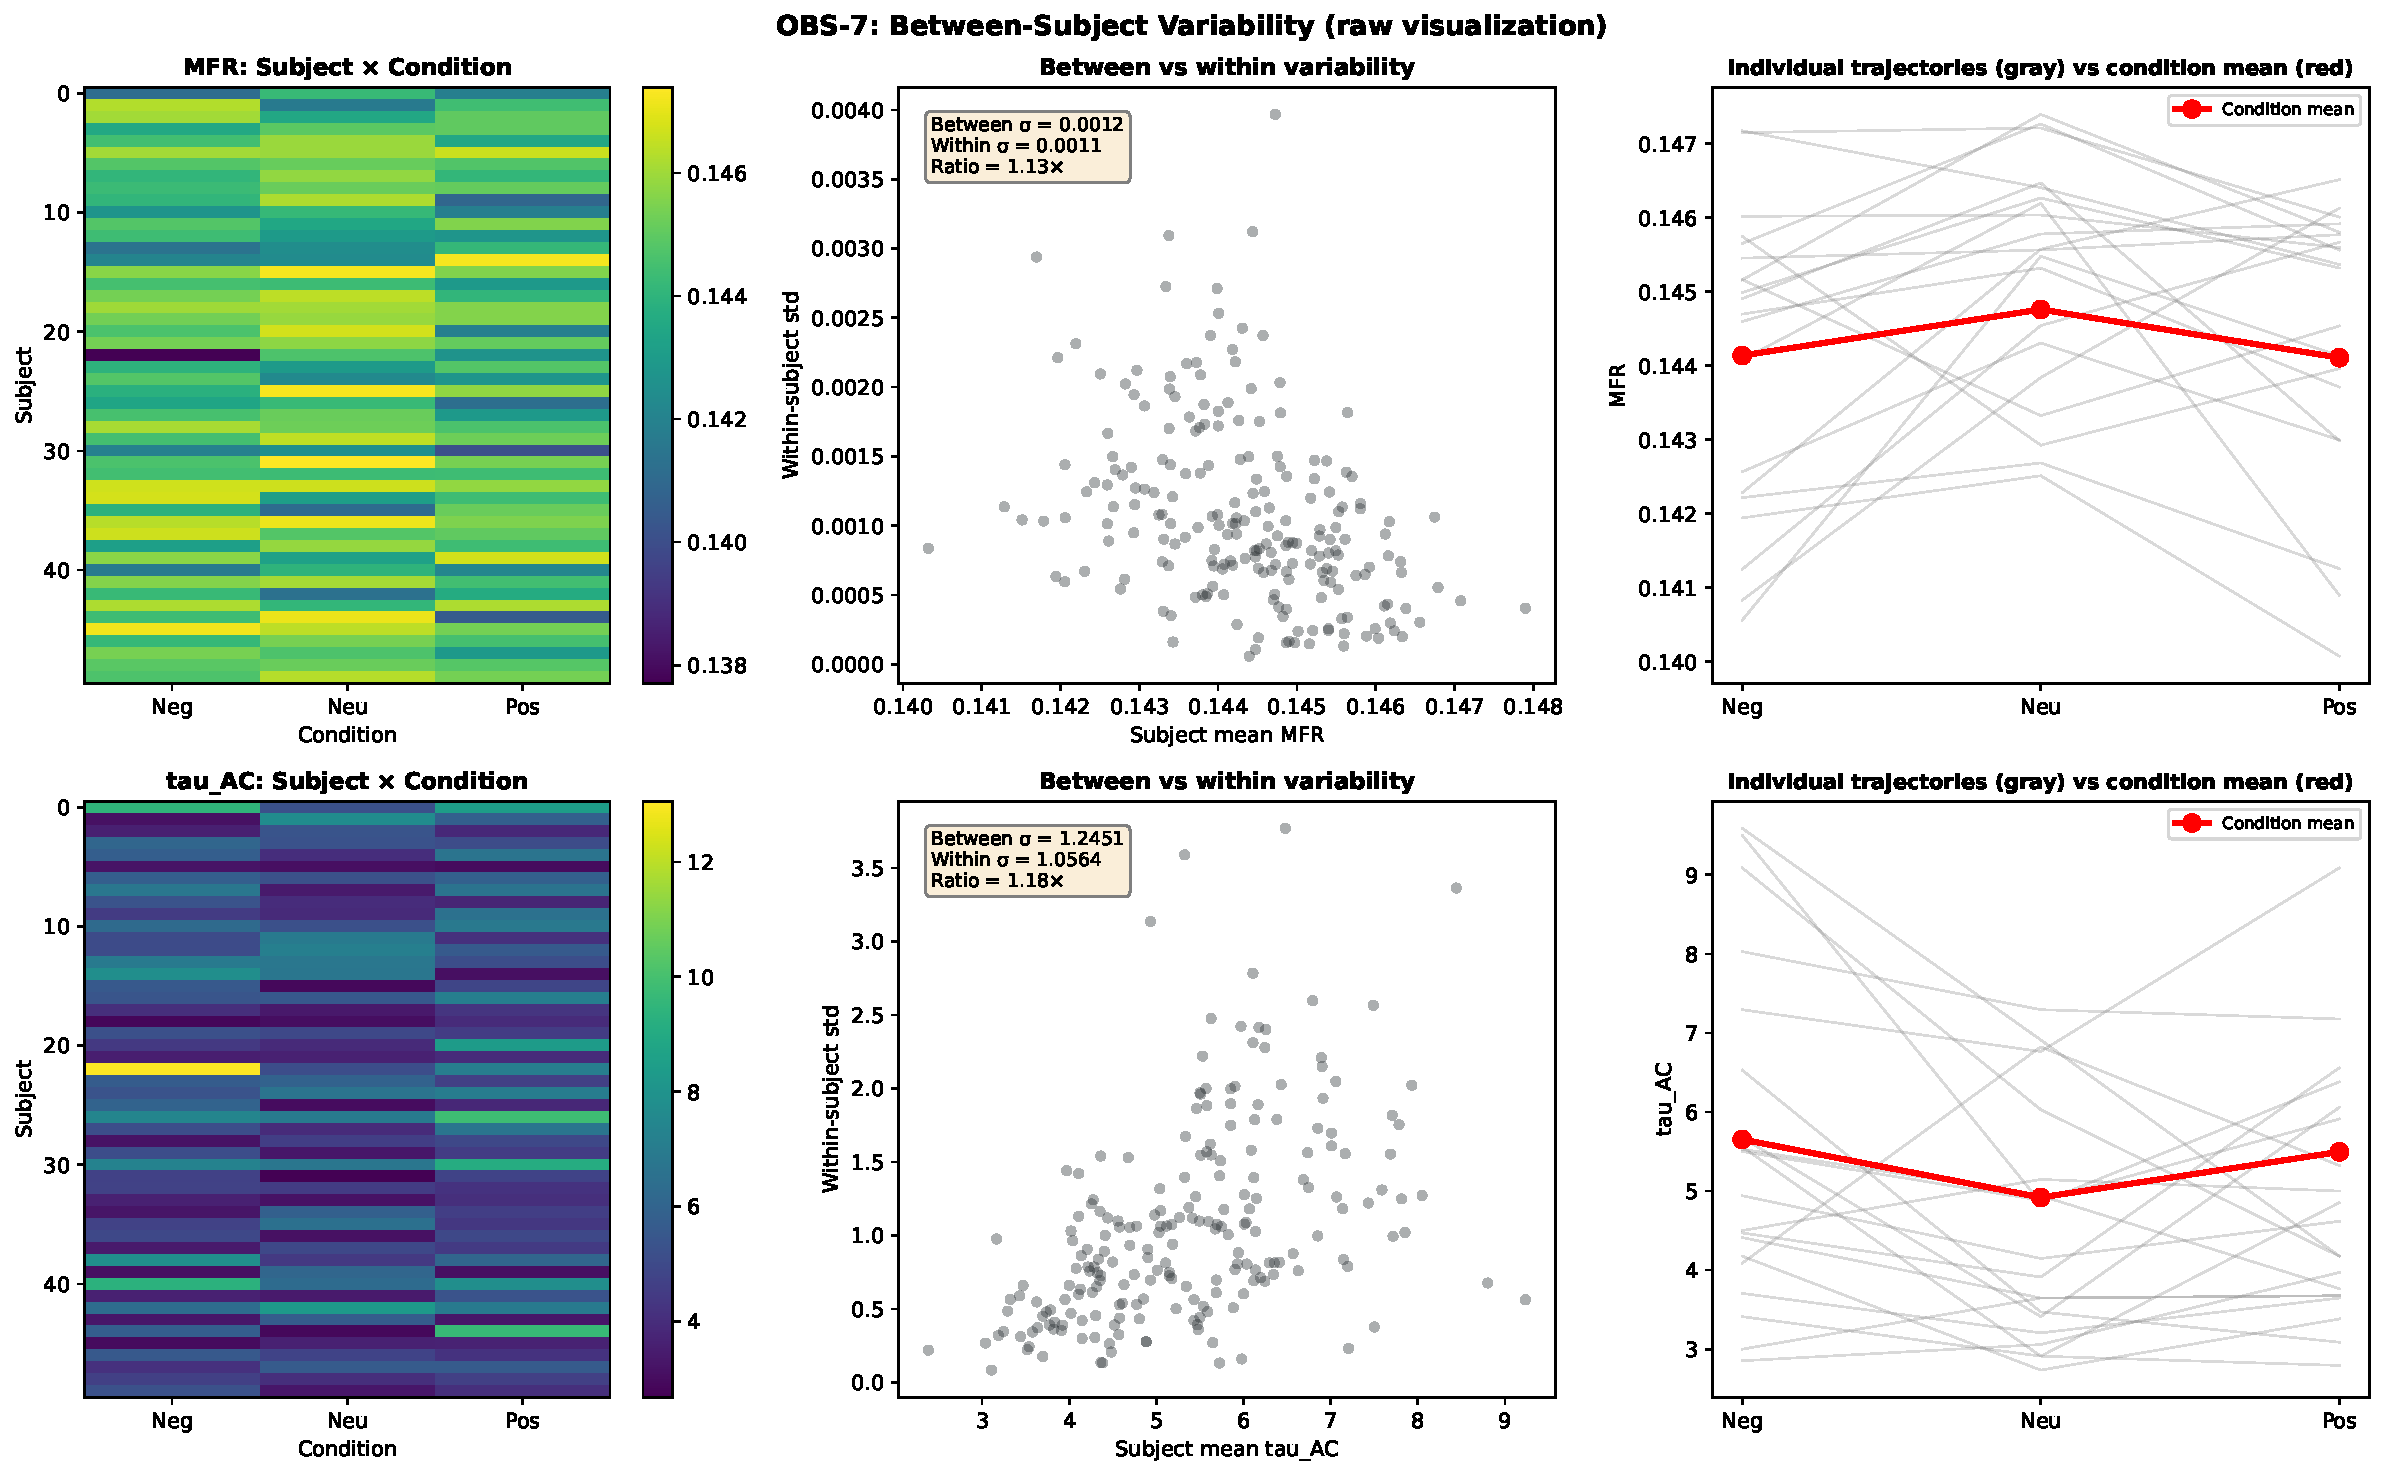
\includegraphics[width=\textwidth]{pictures/appendixA/obs07_subject_variability.pdf}
    \caption{OBS-7: Between-subject versus within-subject variability. Rate entropy and permutation entropy show within-subject variability \emph{exceeding} between-subject variability (ratios $0.87\times$ and $0.90\times$), a fundamentally different variance regime from the BSC$_6$ embeddings ($7\times$ subject dominance). The dynamical metrics are more condition-responsive than subject-dominated.}
    \label{fig:app_ch6_obs07}
\end{figure}

\begin{figure}[H]
    \centering
    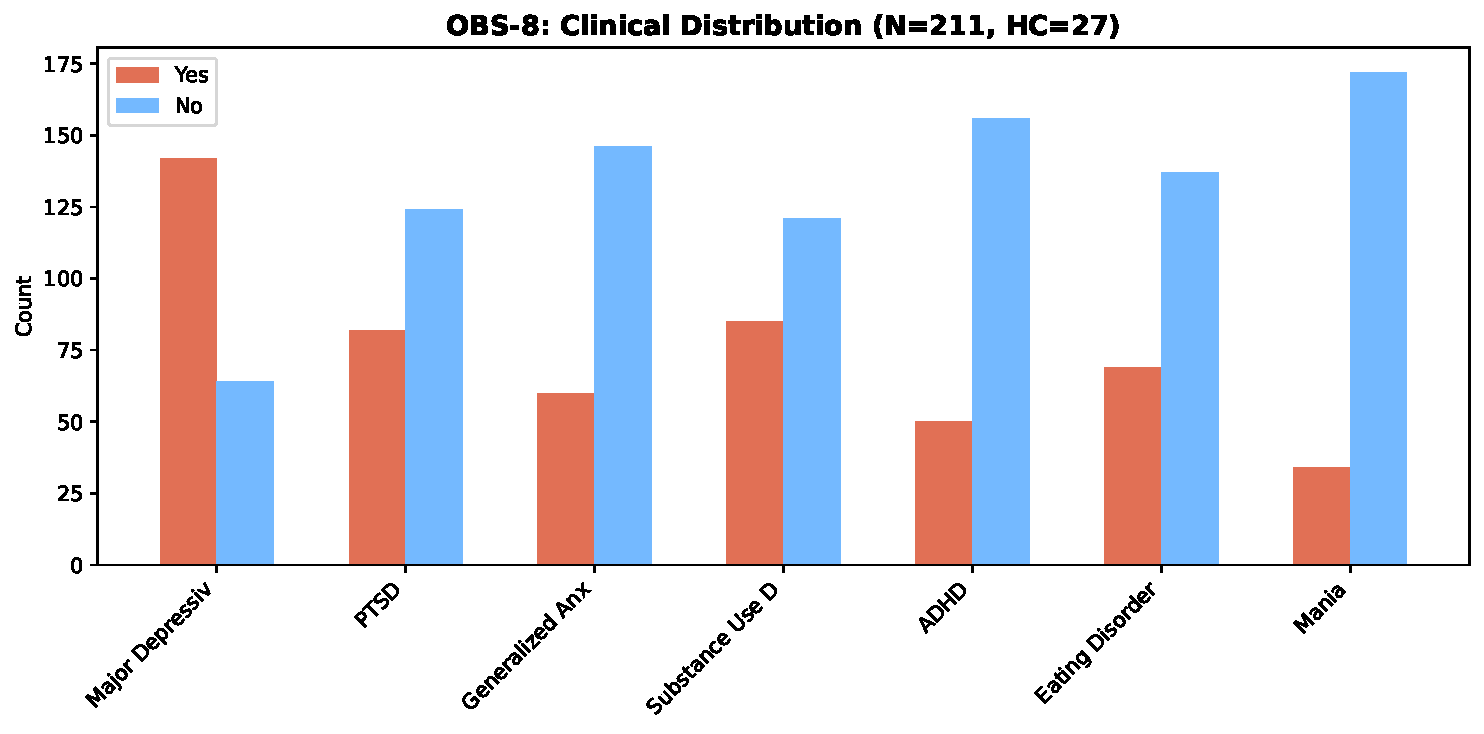
\includegraphics[width=\textwidth]{pictures/appendixA/obs08_clinical_distribution.pdf}
    \caption{OBS-8: Clinical metadata coverage. $206$ of $211$ subjects have diagnostic data. MDD: $142$ vs.\ $64$. PTSD: $82$ vs.\ $124$. SUD: $85$ vs.\ $121$. Healthy controls (zero of five primary diagnoses): $27$. Mean comorbidity: $2.8$ diagnoses per subject.}
    \label{fig:app_ch6_obs08}
\end{figure}



%% ═══════════════════════════════════════════════════════════════
%% SECTION A.5: CHAPTER 7
%% ═══════════════════════════════════════════════════════════════
\section{Chapter 7: Structure-Function Coupling}
\label{app:ch7_figs}

The five three-class coupling experiment figures (EXP-7.1 through EXP-7.5) are presented inline in Chapter~\ref{chap:synthesis}, Section~\ref{sec:ch7_3class}. The fourteen four-class coupling figures are presented inline in Sections~\ref{sec:exp7_coupling}--\ref{sec:exp7_augmentation} of the same chapter. No supplementary coupling figures are required.